%---------------------------------------------------------------------------%
%-                                                                         -%
%-                           LaTeX Template                                -%
%-                                                                         -%
%---------------------------------------------------------------------------%
%- Copyright (C) Huangrui Mo <huangrui.mo@gmail.com> 
%- This is free software: you can redistribute it and/or modify it
%- under the terms of the GNU General Public License as published by
%- the Free Software Foundation, either version 3 of the License, or
%- (at your option) any later version.
%---------------------------------------------------------------------------%
%->> Document class declaration
%---------------------------------------------------------------------------%
\documentclass[twoside]{Style/ucasthesis}%
%- Multiple optional arguments:
%- [<oneside|twoside|print>]% oneside eprint, twoside eprint, or paper print
%- [fontset=<adobe|none|...>]% specify font set instead of automatic detection
%- [scheme=plain]% thesis writing of international students
%- [draftversion]% show draft version information
%- [standard options for ctex book class: draft|paper size|font size|...]%
%---------------------------------------------------------------------------%
%->> Document settings
%---------------------------------------------------------------------------%
\usepackage[authoryear,list]{Style/artratex}% document settings
%- usage: \usepackage[option1,option2,...,optionN]{artratex}
%- Multiple optional arguments:
%- [bibtex|biber]% set bibliography processor and package
%- [<numbers|super|authoryear|alpha>]% set citation and reference style
%- <numbers>: textual: Jones [1]; parenthetical: [1]
%- <super>: textual: Jones superscript [1]; parenthetical: superscript [1]
%- <authoryear>: textual: Jones (1995); parenthetical: (Jones, 1995)
%- <alpha>: textual: not available; parenthetical: [Jon95]
%- [geometry]% reconfigure page layout via geometry package
%- [lscape]% provide landscape layout environment
%- [xhf]% disable header and footer via fancyhdr package
%- [color]% provide color support via xcolor package
%- [background]% enable page background
%- [tikz]% provide complex diagrams via tikz package
%- [table]% provide complex tables via ctable package
%- [list]% provide enhanced list environments for algorithm and coding
%- [math]% enable some extra math packages
%- [xlink]% disable link colors
\usepackage{Style/artracom}% user defined commands
\usepackage[justification=centering]{caption}
%---------------------------------------------------------------------------%
%->> Document inclusion
%---------------------------------------------------------------------------%
%\includeonly{Tex/Chap_1,...,Tex/Chap_N}% selected files compilation
%---------------------------------------------------------------------------%
%->> Document content
%---------------------------------------------------------------------------%
%-
%-> Titlepage information
%-
%---------------------------------------------------------------------------%
%->> Titlepage information
%---------------------------------------------------------------------------%
%-
%-> 中文封面信息
%-
\confidential{}% 密级:只有涉密论文才填写
\schoollogo[scale=0.095]{ucas_logo}% 校徽
\title{隐式几何表达在神经网络渲染和重建中的应用}% 论文中文题目
\author{金石}% 论文作者
\advisor{虞晶怡~教授~上海科技大学}% 指导教师:姓名 专业技术职务 工作单位
%\advisor{指导教师一\\指导教师二\\指导教师三}% 多行指导教师示例
\degree{硕士}% 学位:学士、硕士、博士
\degreetype{工学}% 学位类别:理学、工学、工程、医学等
\major{通信与信息系统}% 二级学科专业名称
\institute{中国科学院上海微系统和信息技术研究所}% 院系名称
%\institute{中国科学院力学研究所\\流固耦合实验室}% 多行院系名称示例
\date{2021~年~6~月}% 毕业日期:夏季为6月、冬季为12月
%-
%-> 英文封面信息
%-
\TITLE{Application of implicit geometric representation in neural rendering and reconstruction}% 论文英文题目
\AUTHOR{Jin Shi}% 论文作者
\ADVISOR{Supervisor: Professor Yu jingyi}% 指导教师
\DEGREE{Master}% 学位:Bachelor, Master, Doctor, Postdoctor。封面据英文学位名称自动切换,需确保拼写准确
\DEGREETYPE{Science in Engineering}% 学位类别:Philosophy, Natural Science, Engineering, Economics, Agriculture 等
\MAJOR{Communication and Information System}% 二级学科专业名称
\INSTITUTE{Shanghai Institute of Microsystem and Information Technology, Chinese Academy of Sciences}% 院系名称
\DATE{June, 2021}% 毕业日期:夏季为June、冬季为December
%---------------------------------------------------------------------------%
%
\begin{document}
%-
%-> Frontmatter: title page, abstract, content list, symbol list, preface
%-
\frontmatter% initialize the environment
%---------------------------------------------------------------------------%
%->> Frontmatter
%---------------------------------------------------------------------------%
%-
%-> 生成封面
%-
\maketitle% 生成中文封面
\MAKETITLE% 生成英文封面
%-
%-> 作者声明
%-
\makedeclaration% 生成声明页
%-
%-> 中文摘要
%-
\intobmk\chapter*{摘\quad 要}% 显示在书签但不显示在目录
\setcounter{page}{1}% 开始页码
\pagenumbering{Roman}% 页码符号

虚拟现实(VR)和增强现实(AR)技术的发展使得数字化真实世界成为学术和工业探索的热点,人和物体的几何表达是其中重要的技术环节。 几何表达有多种数学形式和数据结构,在不同的应用中各有优劣。近年来深度学习已经应用到几何重建和渲染中,同样需要选取特定几何表达形式作为中间件。本文讨论将隐式几何表达结合到深度学习的统一框架,以编解码器为核心结构,将输入数据经编码器变换到特征空间,接着将特定的隐式几何表达嵌入到网络中,同时把数学物理过程表达成神经网络的计算图。最终根据特定任务,设计输出层。为了说明该思想,以多视角图片视角插值渲染和点云重建这两个任务为例。对于视角插值渲染,将传统的两视角线性插值革新为以三视角为核心的圆环上的插值模型,以基于视差的隐式几何作为神经网络解码器的输出,并辅以可视化区域的预测,同时将插值计算过程写成可导的神经网络层,构建了基于编解码器结构的插值网络。在人体数据集和一般物体数据集上的实验表明效果明显优于之前的方法。对于点云重建,借助可导渲染将点云投影到多视角并经编码器变换到特征空间,将解码器赋予隐函数的物理意义,用以预测空间任意点的隐函数值,通过提取等值面生成几何模型。在多个数据集上的实验表明新方法提高了点云重建对噪声的鲁棒性和重建效果。通过两个具体应用突出了隐式表达既能精确描述模型的几何,又具备连续可导等性质,适合与深度学习技术结合,实现数据先验与经验知识的结合。

本文的主要贡献如下:
\begin{enumerate}
\item 设计了结合隐式表达的深度学习框架用以表达和学习几何信息。
\item 在自由视角插值的应用中,基于引入的隐式表达形式,提出了基于三相机的环形插值模型和相应的矫正算法,革新了之前的两相机插值模型。
\item 在点云重建的应用中,基于引入的隐式表达和深度学习框架,提出将点云先通过点投影的方式进行多视角的2D网格化,再预测隐式表达形式的方法,适用于单视角和多视角的情形,提高了点云重建的鲁棒性。
\end{enumerate}




\keywords{隐式表达,三维重建,自由视角插值,神经渲染}% 中文关键词
%-
%-> 英文摘要
%-
\intobmk\chapter*{Abstract}% 显示在书签但不显示在目录

With the development of virtual reality (VR) and augmented reality (AR) technology, digitalizing the real world has become a hot topic in both academy and industry. The geometry of human body and general objects is an important technique. There are many mathematical forms and data structures for geometry, which have their own advantages and disadvantages in different applications. In recent years, deep learning has been applied to 3D reconstruction and rendering, and it also need to select specific geometric representation as middleware. This paper discusses a unified framework that combines implicit geometric representation with deep learning. With a core encoder-decoder structure, the input data is transformed to feature space through encoder, and then the specific implicit geometry is embeded into the network. At the same time, the mathematical and physical process is represented as the computation graph of neural network. Finally, the output layer is designed according to the specific task. In order to illustrate the idea, this paper discuss two specific applications: view morphing and point cloud reconstruction. For view morphing, the traditional two-view linear interpolation is replaced by the new three-view cyclic morphing framework. Parallax is chosen as the output of the decoder, at the same time the visual mask is predicted. The interpolation process is implemented as a differential layer. Experiments on human body data and general object show that the performance is better than the previous methods. For the pointcloud reconstruction, the pointcloud is rendered to multiple views and encoded to the feature space. The decoder is expected to be the implicit function of the underlying true geometry, it can predict the isovalue of any point in the 3D space. The mesh is extracted using marching cubes algorithm. Experiments on several datasets show that the new method improves the robustness to noise and also the reconstruction performance. Through the two specific applications, it shows that implicit geometric representation is accurate with continuous derivative. It is suitable to combine with deep learning to acquire the data prior and empirical knowledge at once.

The contribution of this thesis is summarized as follows:
\begin{enumerate}
\item This thesis designs a learning-based framework combining implicit geometric representation, to encode and learn geometric information.
\item In the application relating to free-viewpoint interpolation, this thesis proposes a cyclic triplet-camera model for interpolation and rectification, which is a key improvement to the previous two-camera model.
\item In the application relating to pointcloud reconstruction, this thesis proposes a pipeline of multi-view 2D rasterization followed by point-based projection, to encode the feature of pointcloud for later implicit geometry prediction. This pipeline applies to both cases of single view or multiple views, which attains better robustness than previous methods.
\end{enumerate}

\KEYWORDS{Implicit representation, 3D Reconstruction, Free viewpoint interpolation, Neural rendering}% 英文关键词
%---------------------------------------------------------------------------%
% title page, abstract
{% content list region
\linespread{1.2}% local line space
\intobmk*{\cleardoublepage}{\contentsname}% add link to bookmark
\tableofcontents% content catalog
\intobmk*{\cleardoublepage}{\listfigurename}% add link to bookmark
\listoffigures% figure catalog
\intobmk*{\cleardoublepage}{\listtablename}% add link to bookmark
\listoftables% table catalog
}
%%%% \intobmk\chapter*{符号列表}% 显示在书签但不显示在目录

\section*{字符}
\nomenclatureitem[\textbf{Unit}]{\textbf{Symbol}}{\textbf{Description}}
\nomenclatureitem[$\Unit{m^{2} \cdot s^{-2} \cdot K^{-1}}$]{$R$}{the gas constant}
\nomenclatureitem[$\Unit{m^{2} \cdot s^{-2} \cdot K^{-1}}$]{$C_v$}{specific heat capacity at constant volume}
\nomenclatureitem[$\Unit{m^{2} \cdot s^{-2} \cdot K^{-1}}$]{$C_p$}{specific heat capacity at constant pressure}
\nomenclatureitem[$\Unit{m^{2} \cdot s^{-2}}$]{$E$}{specific total energy}
\nomenclatureitem[$\Unit{m^{2} \cdot s^{-2}}$]{$e$}{specific internal energy}
\nomenclatureitem[$\Unit{m^{2} \cdot s^{-2}}$]{$h_T$}{specific total enthalpy}
\nomenclatureitem[$\Unit{m^{2} \cdot s^{-2}}$]{$h$}{specific enthalpy}
\nomenclatureitem[$\Unit{kg \cdot m \cdot s^{-3} \cdot K^{-1}}$]{$k$}{thermal conductivity}
\nomenclatureitem[$\Unit{kg \cdot m^{-1} \cdot s^{-2}}$]{$S_{ij}$}{deviatoric stress tensor}
\nomenclatureitem[$\Unit{kg \cdot m^{-1} \cdot s^{-2}}$]{$\tau_{ij}$}{viscous stress tensor}
\nomenclatureitem[$\Unit{1}$]{$\delta_{ij}$}{Kronecker tensor}
\nomenclatureitem[$\Unit{1}$]{$I_{ij}$}{identity tensor}

\section*{算子}
\nomenclatureitem{\textbf{Symbol}}{\textbf{Description}}
\nomenclatureitem{$\Delta$}{difference}
\nomenclatureitem{$\nabla$}{gradient operator}
\nomenclatureitem{$\delta^{\pm}$}{upwind-biased interpolation scheme}

\section*{缩写}
\nomenclatureitem{CFD}{Computational Fluid Dynamics}
\nomenclatureitem{CFL}{Courant-Friedrichs-Lewy}
\nomenclatureitem{EOS}{Equation of State}
\nomenclatureitem{JWL}{Jones-Wilkins-Lee}
\nomenclatureitem{WENO}{Weighted Essentially Non-oscillatory}
\nomenclatureitem{ZND}{Zel'dovich-von Neumann-Doering}

% symbol list, preface content
%-
%-> Mainmatter
%-
\mainmatter% initialize the environment
%---------------------------------------------------------------------------%
%->> Main content
%---------------------------------------------------------------------------%
\chapter{引言}\label{chap:introduction}

\section{研究背景}
从图像中恢复三维几何是计算机视觉需要解决的根本问题之一,针对不同物体的几何重建,在工业和商业上有诸多应用。随着虚拟现实(Virtual Reality, VR)和增强现实(Augmented Reality, AR)硬件设备的工业流程进步,诸如线上购物、虚拟看房、场景融合等应用对物体的几何恢复有很紧迫的需求,而针对人的几何重建在虚拟试衣、数字人以及全息视频等应用中属于关键技术。由此可见几何重建的好坏将对未来的教育、电商、沟通等诸多方面有着相当大的影响。

工业界当前用于几何建模的生产工具主要以面片和经典参数化曲线作为几何的表达形式,这些传统的几何表达方式有着利用手工编辑、存储规范以及适配渲染贴图等流程的优点。但是随着模型几何生成的自动化程度提高,人工编辑的工作量在下降,只需对算法生成的结果进行部分修正,而传统的面片表达形式对瑕疵过于敏感,少许几何上的瑕疵可能极大影响观赏体验,使得算法自动生成模型的优势无法体现。另一方面随着深度学习在三维重建方面的应用,越来越多的研究工作将人和物体的重建建模成一个连续可导的过程,而面片表达本质上为离散图结构,显然不是与神经网络结合的最佳选择。不仅如此,近年来涌现出的诸多可导渲染器对材质和贴图的表示方法也提供了新的可能,这同样使得以面片和参数化曲线表达的建模方式不再是必须的。

三维几何除开本身作为独立的研究目标,还与其余诸如渲染、自由视点、材质光照估计等领域有着紧密联系。所有与3D视觉相关的问题,都绕不开选取适当的几何表达作为中间件这一过程。在光场渲染中常常需要较为粗糙的几何模型作为先验,使得渲染出来的图片或视频具备一定的视角依赖性,以提高真实感。在自由视点插值中,同样需要几何来提供图片之间的像素对应关系。相比于得到高质量的几何模型,在这些问题中更加关注最终呈现出来的图片和视频的质量,而允许作为中间件的几何模型有一定的瑕疵,这使得对几何表达形式的选取变得更加微妙。

近年来深度学习与3D视觉结合的方法在诸如单视角恢复几何(Single View Reconstruction, SVR)、多视角重建(Multi-View Stereo, MVS)以及神经渲染(Neural Rendering, NR)等诸多方面取得了超越之前传统方法的结果\citep{jiang2020sdfdiff, mildenhall2020nerf, park2019cvpr, saito2019pifu, meshcheder2019cvpr}。这些工作开始探索将包括传统的面片、体积离散以及隐函数等形式的几何表达融合进深度学习的框架中,而在这些表达中,相比于以面片为主的显式表达,隐式几何表达明显更适合深度学习框架下的3D视觉任务。


\section{研究现状}
围绕几何重建的工作包括关注几何本身的和应用几何信息作为中间件来达到渲染以及视角生成等目的的工作,而这些问题本身的输入来源又多种多样。本文讨论的工作局限于从二维的图像得到三维信息,以下按照应用目的分类进行几个方面的研究现状综述。

\subsection{多视角图片的重建}
在人物重建和物品重建方面,多视角重建用来生成完整的带贴图的三维模型,采集系统的搭建非常复杂,常常需要多达几十甚至上百的相机进行同步拍摄。早期的工作包括从轮廓信息重建\citep{vlastic2008, furukawa2006, matusik2000ibvh},将2D图片中提取的轮廓投影成空间中的可见视锥区域并对所有的可见区域求交集“切”出最终的模型。这种方法在图片数量足够的情况下能获得不错的几何,但是无法处理非凸的情形。精细的几何和纹理信息就要依赖于多视角立体匹配约束\citep{furukawa2010, starck2007, zitnick2004},这些方法利用多视角图片中特征点的匹配,计算出稀疏点云或者分层的深度图来作为几何表达,在此基础上生成密集点云以及进行补全和去噪,再将点云用泊松重建\citep{kazhdan2013, kazhdan2006}等方式恢复成面片。多视角设定下通过可控地改变光照条件拍摄多张照片也能恢复出几何\citep{wu2012, vlasic2009},这类方法通过恢复像素级的法向信息来估计几何,精度较高,但是对光源搭建和拍照环境的要求较高,对于非朗伯表面的物体诸如金属等反光材质的效果无法保证。

在多视角的设定下用深度学习框架来生成3D表面的工作集中在将传统的特征提取和匹配框架换成完全可导的连续过程。三维网格是这类方法中一种典型的表达几何的形式,\citet{ji2017iccv}通过计算离散网格的代价函数,并据此对每个格点指定对应的视角图片,并用3D卷积网络来对网格是否属于表面进行回归。\citet{kar2017neurips}通过可导的投影和反投影算子,将图片中的特征融合到三维网格中,以此为依据对网格进行分类。另一类工作试图利用深度学习对数据的学习能力,来降低所需图片和视角的数量,以达到稀疏多视角设定下高质量的三维重建,这有利于减轻多视角拍摄系统的搭建,节省大量成本,意义非常重大。通过使用轮廓信息得到粗糙的几何模型再利用颜色信息和网络去细调,来得到高精度的模型\citep{Gilbert_2018_ECCV,huang2018eccv},本质上能减少输入的视角数量,是由于训练时使用了高精度模型作为监督。所有这些基于三维网格的几何表达方式都难以避免内存开销巨大的弊病,因此无法适用于大型场景,同时只能在低分辨率网格上表达粗滤的几何结构。\citet{yao2018mvsnet}使用深度图的形式表达几何,减少了内存开销,最终的重建结果由深度图反投影的点云表示,但是在网络中还是使用了离散网格表达相关的度量张量。

对存储依赖真正减少的契机出现在\citet{meshcheder2019cvpr}提出用多层感知机(Multi-Layer Perceptron, MLP)来表达几何,通过一个MLP网络对空间中任意点在表面内部还是外部进行分类,而最终的表面则通过两类区域的边界构成,数学上这就是图形学领域早就存在的使用隐函数来表达几何。仅仅预测点在表面的内部还是外部形式无法应用隐函数更多的几何和代数性质,一些工作干脆将有符号距离场(Signed Distance Function, SDF)引入到深度学习框架中\citep{jiang2020sdfdiff, park2019cvpr},同样使用MLP表示。SDF是一个表达空间中任意点到表面距离的函数,同时距离的符号表达在面的内部还是外部,由于其在表面附近拥有关于法向的良好性质,有助于提升表面的重建细节。\citet{yariv2020multiview}使用SDF表达结合由向量表达的材质信息,使用球追踪(Sphere Tracing)方法进行可导渲染的方式来同时分离并重建几何和材质信息,取得了很好的效果。

\subsection{单视角图片的重建}
单视角的重建根据场景不同有很大区别,若物体为静态且基本上符合朗伯表面的假设,则可以移动相机等效于在多个视角同时拍摄,把问题转化为多视角重建。真正意义上的单视角重建实际上针对的是单张图片或者是视频,而根据相机类型的不同,又可以进一步加以分类。\citet{newcombe2011kfuse}提出了以深度图流为输入的实时重建算法,该方法拉开了以颜色加深度为输入进行实时重建的序幕,同时确立了以配准和融合交替进行为框架的算法框架,其中配准过程是将模型对齐到当前数据,融合是以截断的SDF为几何表达进行模型更新的过程。这里展示出了SDF另一条突出的性质:与传统面片表达不易修改拓扑关系的弱点相比,SDF能够通过连续的迭代过程,平滑地对几何进行变换,包括拓扑变化。同时SDF的隐式几何能迅速地转化为面片\citep{lorensen1987}。然而仅仅是刚性场景的重建只能表达静态的情况,单相机模型中往往要对时序数据进行处理,动态场景变得非常常见,显而易见以采集人体为例,要求人在几十秒至数分钟的采集时间内纹丝不动过于苛刻。\citet{zollhofer2014}提出了对一般性物体的非刚性实时重建算法,将非刚性的迭代最近点算法(Non-rigid ICP)与融合过程结合在一起。自此开始的非刚性实时重建算法在配准的计算过程和目标函数设计上有诸多变化\citep{slavcheva2017, dou2016, innmann2016volume, newcombe2015},有的基于三维网格的形变,有的基于面片简化后的拓扑图进行计算,但是融合过程始终还是用截断SDF表达。但是基于深度信息的重建算法对实现要求很高,算法复杂,鲁棒性差,同时考虑到实际应用中以手机相机最为普及,而当时手机摄像头还未配置深度相机,这使得研究者们开始思考绕开深度信息以及配准加融合的算法框架,仅考虑彩色图片和视频的输入。

基于彩色图片或者视频进行重建是非常病态的问题,约束条件太少,这就使得求解必须依赖于足够充分的先验知识或者假设。由于基于人体的参数化模型研究基础比较充分\citep{loper2015smpl, anguelov2005scape},很多工作将问题转化为从图片估计模型参数。这类方法中,图片的轮廓信息、关节点信息\citep{cao2019openpose, fang2017rmpe}以及其他一些手工标注的信息,常常被用来初始化拟合参数\citep{zhou2010, guan2009}。近年出现了设计深度学习框架直接端到端去预测模板参数的方法\citep{Pavlakos_2018_CVPR, kanazawa2018},提高了对一些极端遮挡情况的鲁棒性,同时能够融入诸如人体分割信息这样本身就适合深度学习的子任务联合训练\citep{omran2018nbf},获得更好的效果。\citet{alldieck2018video}对视频输入通过优化多帧共同的形状参数和逐帧的姿态参数,求解时间序列上的连续模板参数,并通过轮廓进行细节的调优。但是参数化模型本身仅仅是表达了一个赤裸的人体,对于穿紧身衣服的情况还能适用,但是对于比较宽松的衣服、裙子以及头发或者是手上提了东西的情景就无法表达了。因此研究者们开始回归到无模板的方法,\citet{varol2018}提出了直接学习一个固定分辨率的三维网格的方法,但是由于网格消耗内存的缘故,几何的细节完全丢失掉了。与多视角情形相似,隐函数的引入解决了存储消耗的问题。\citet{saito2019pifu}提出了将隐函数形式与像素对齐的方法,通过将特征张量投影到像素空间来建立几何与图片像素之间的数学模型,并通过大量高精模型与图片构成的数据对进行学习,同时这个框架还能推广到多视角的情形。该工作不久又通过引入法向图的预测并由此对几何模型进行细调,而得到了精度和纹理更加好的结果\citep{saito2020pifuhd}。\citet{Chibane_2020_CVPR}同样采用隐函数的形式,与前面不同的在于不仅考虑一个点或者像素,而是对包含一个点的局部空间进行整体考虑,将这个局部空间离散成一个不大的网格作为输入,文章提出的方法适用于多项任务。

\subsection{神经网络表达的视角生成}
视角生成本身属于一个独立的研究领域,很多基于图像渲染的工作专门绕开几何信息而直接试图合成新的视角图片,与本文关注几何的根本出发点无关,在此并不综述这方面的文章。另一些视角合成的工作则是将几何表达作为中间件,通过选取特定的几何表达形式,来更好地提取和融合图片中的3D信息,最后再将目标锁定在合成的图片质量上,而作为中间件的几何质量并不在直接的考量范围之内。但是即便是带几何的视角合成工作数量也很庞大,本文在此仅关注结合了深度学习以及和神经渲染相关的视角生成工作。

卷积神经网络最初被引进视角合成的任务时并没有考虑几何表达,而是仅仅利用卷积的结构去拟合数据集来完成新视角合成\citep{TDB16a}以及帧间插值等\citep{niklaus2017}。\citet{jaderberg2015}提出了往卷积网络里面接入可导模块进行几何变换,这才使得在网络中加入几何相关的表达成为可能。\citet{flynn2016}使用深度图来融合网络预测出的不同深度的图片,\citet{kalantari2016}使用视差来表达几何对光场数据做新视角的合成,\citet{zhou2016view}使用光流作为中间件来预测输入图片到新视角图片的像素之间的关系,\citet{tvsn_cvpr2017}同样使用光流作为几何表达,但是为了解决遮挡区域的补全问题,又引入了对抗网络通过学习数据的分布来猜出遮挡区域更真实的像素信息。不难发现,这些方法里面的几何表达方法全都是隐式的表达,与3D的隐函数表达不同,这些几何表达方式已经被离散到2D网格上并于像素对齐,能够更好地利用卷积网络感知局部信息的优势。但是卷积网络基本上只能对于图片做整体的卷积操作,生成的图像往往有模糊和振铃等瑕疵,细节也很难恢复。

最近的工作开始从光线的角度重新考虑视角合成,这类工作通常用网络来表达隐式几何,输入空点中点的位置和光线方向,网络则输出诸如SDF函数值或者其他的隐函数值,并以此逐根光线地渲染出整幅图。\citet{sitzmann2019srns}使用LSTM来对场景中每个空间中的连续点进行编码,提却特征并模拟光线追踪的过程来渲染图片。\citet{mildenhall2020nerf}借鉴了烟雾的几何表达,使用一个MLP来预测空间点的密度,同时预测与视角关联的光线上各点的颜色值,并用采样离散点结合体渲染的方式渲染出最终的颜色。\citet{oechsle2020}使用网络从输入图片中表达场景的表面光场,并同时恢复光照信息,使得可以实现带重打光功能的新视角合成。


\section{本文研究的问题}
从研究现状的分析中可以发现,基于图片的三维重建技术本身以及以几何作为中间件的渲染和图片生成领域,都已经和深度学习技术框架广泛结合。隐式几何表达不仅具备可导性,其针对具体应用的表达形式对存储需求的调整灵活度还很高。因此本文的注意力放在隐式几何表达与深度学习框架的结合上,结合视角插值和点云重建两个具体的应用进行研究。

对于静态场景的视角插值,传统方法的重点与立体匹配类似,主要分为寻找两张图之间的密集特征匹配和插值融合两步\citep{seitz1996}。\citet{Ji_2017_CVPR}将传统框架变成了基于深度学习的可导框架,但是遮挡变化、大相机基线下的插值以及多张图之间的连续变化这些问题并没有解决。本文针对这些缺陷,设计了新的三相机视角插值框架。包含了新的预矫正模型,对多张图之间的连续插值有逼近二阶连续的轨迹,同时引入了基于视差的隐式几何表达作为中间件,可以导出图片之间的密集特征,最终通过带有效区域加权的可导融合方法合成新视角的图片。通过在一般物体的数据集\citep{shapenet2015}和人体数据集\citep{varol2017}上进行了训练和与其他方法的对比,证明本文的新方法对于遮挡造成的歧义能够比较好的消除,合成高质量的连续中间图片。新的框架还支持通过连续插值产生360度的“子弹时间”效果,而这一切背后的支撑主要在于隐式几何的选择,和据此进行的误差函数的设计。

对于点云重建的任务,目标主要是从粗糙的点云恢复出显式几何,这些输入点云的来源有多种可能,往往是带噪声和空洞等几何缺陷、同时分辨率可能还偏低的扫描数据。经典传统方法当属泊松重建\citep{kazhdan2013, kazhdan2006},对点云的重建仅仅利用局部数据的位置和法向信息进行,相当于无任何先验的空间上的插值。本文提出的方法基于深度学习框架,将离散的点云转化为隐函数的形式,并在此基础上进行补全和去噪,最终提取显式几何。对于点云本方法首先通过可导渲染的方式将点云编码成多视角的图像形式,用MLP代表隐函数,输入空间点的位置信息和从点云中提取的特征,预测隐函数的输出值。通过在两个不同的人体数据上的训练与测试\citep{muller2009},本方法能够同时利用点云数据本身的信息以及从高精度数据中学习到的信息,生成去噪和补全后的模型,并能够保留更多的几何细节,说明了隐式几何表达结合深度学习在该任务上的优势。

\section{本文的组织结构}
本文工作包含两个基于隐式几何在具体任务上的应用,本文余下内容将分别阐述两个任务的方法以及实验结论。本文的组织结构如下:

第二章介绍环形三相机视角变换的方法。主要包含算法模块中的各个部分的原理介绍与讨论,即环形矫正算法、编解码器神经网络的设计、可见区域的预测以及视角融合生成模块以及目标函数的设计。

第三章介绍环形三相机视角变换方法的实现与实验结果,以及与其他基于深度学习的视角生成算法的比较。

第四章介绍基于隐函数的点云重建方法。包括从点云可导渲染到多个视角的过程,二维上的特征提取与补全,隐函数模块的预测与目标函数的设计方案。

第五章介绍基于隐函数的点云重建实现方式、训练数据的准备和实验结果,并与传统泊松重建结果的比较。

第六章对工作进行总结和展望,对隐式几何在深度学习框架下对重建和渲染的效果进行总结,并指出未来继续改进甚至在实际生产中应用的前景。
\chapter{环形三相机视角插值方法}\label{chap:CVM_method}
视觉特效由于提供了独特的观赏体验,已经成为影视作品不可或缺的一部分。最著名的例子之一是《黑客帝国》中呈现的“子弹时间”效果。它创造了时间暂停的错觉,让观众似乎围绕演员转了一圈,并且视点平滑过渡。为了产生这种效果,160多个摄像头被同步和精确排列,这些相机通过一套高精度的激光对准系统在拍摄轨道上对齐,形成穿过空间的复杂拍摄曲线。然而,这种专门的采集系统造价昂贵,需要付出巨大的努力来建造。

视角插值算法能够使得“子弹时间”效果的建立更加灵活,\citet{seitz1996}在这方面的开创性工作指出,通过对两幅图像进行校正后再线性插值,能够实现保形的变换,如图~\ref{fig:view_morphing}。其中校正算法主要是为了降低像素匹配搜索的计算量,将匹配过程的搜索空间从二维降到一维。利用视角插值技术能大大降低使用相机的数量,只需要在轨迹上采样一定数量的相机,然后对每一对相邻的视图进行插值得到中间的帧。
现在考察相邻的两张图,整个视角插值的过程本质上还是需要从两幅图中推测3D几何信息。现有的方法中使用到的几何表达主要有轮廓信息、深度图和光流。这里对相邻图片要求要有较大的重叠区域,才能确保可靠的三维重建和插值。
\begin{figure}[!htbp]
    \centering
    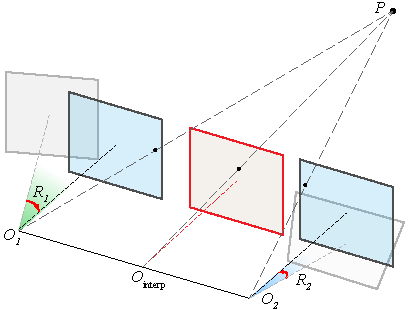
\includegraphics[width=0.60\textwidth]{view_morphing_fig1.pdf}
    \bicaption[视角插值过程示意图]{视角插值过程示意图。$O_1$,$O_2$代表两个相机的光心,$O_{\mathrm{interp}}$代表插值出的虚拟相机光心位置,两幅图像经过$R_1$,$R_2$旋转校正后能够线性插值出$P$在虚拟相机中的投影。}[Process of view morphing between two cameras]{Process of view morphing between two cameras.$O_1$,$O_2$ represent the principle point of input cameras, $O_{\mathrm{interp}}$ represents the virtual camera. After being rectified by $R_1$, $R_2$, the two rotation matrices,  The two reference cameras linearly interpolate the projection of $P$ in the virtual camera.}
    \label{fig:view_morphing}
\end{figure}
\citet{Ji_2017_CVPR}将视角插值的整个过程第一次端到端地放进了深度学习框架,利用训练数据中的冗余模式让网络自己学到了对图片的校正参数和匹配信息。但是到目前为止,这些方法还是一致假设相机路径为线性,并没有成功地展示360度的子弹时间效果。

本文中提出了一种新的同样基于深度学习,设计了能平滑且真实地进行视角变换的框架。这种方法使用最少三个参考图像沿圆弧形路径进行变换,如图~\ref{fig:real_setup}所示。
\begin{figure}[!htbp]
    \centering
    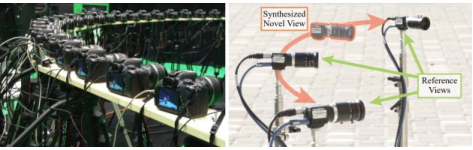
\includegraphics[width=\textwidth]{real_setup.pdf}
    \bicaption[采集系统]{采集系统。左边是需要大量相机的传统子弹时间采集系统示意图,右边是本文提出的方法的采集系统,在一个弧形路径上一组稀疏相机用来采集图像生成视角插值变换后的效果。}[Capturing system]{Capturing system. Left specialized acquisition system with numerous cameras is often needed forproducing the bullet-time effect; right shows the proposed method to morph transition images on acircular path from a sparse set of view samples for rendering such effect.}
    \label{fig:real_setup}
\end{figure}
本文采用了一种新的环形校正技术来将输入的三张图像校准到一个公共圆上,环形矫正后的图像具有最小投影失真的性质。然后将校正后的三张图喂给神经网络,用于新视图合成。本文提出的这个新的网络包含一个编解码结构,用于同时预测像素级运动场和可见性蒙版,还包含一个用于图像插值的混合网络。其中这个运动场和可见性蒙版共同构成了隐式几何表达。与传统的两张图像作为输入不同,本文通过使用第三张中间图像,可以可靠地处理遮挡和大面积的图像视角变化,其中最大的视角变化高达120度。

\section{环形校正}
传统的水平校正在立体匹配中很常见,能将对应匹配的搜索空间缩小到1D水平扫描线,这是因为校正后的图像可以认为是两个完全平行的摄像头直接拍摄得到的。但是这种方法对于围绕着一个物体进行拍摄的场景并不是适用,对于使用三张图片作为输入的情况也不是最优的。原因在于如果使用两两校正,那么三幅图像需要两两进行校正,那么对于一个相机来说会得到多个参数;另一个原因就是对于角度相差较大的两个相机,校正后边界可能出现较大的投影畸变。

本节提出新的环形校正方案,变换三张图像使得它们好像是由三个相机朝向一个公共圆的圆心拍摄的。由于三个不共线的点会确定出一个外接圆,那么总是可以从三个相机的光心坐标计算出这个圆。经过这样的变换后,像素的匹配同样被限制在一维的线上,不过这个线不再是水平。在接下来的过程中使用神经网络实现匹配过程,并将线扫描的约束加到了神经网络的训练中,以增加匹配精度。    

给定三张参考图像$\{\mathcal{I}_l, \mathcal{I}_m, \mathcal{I}_r\}$,以及相机的标定参数$\{K_i, R_i, t_i | i=l, m, r\}$,其中$K_i$是内参矩阵,$R_i$和$t_i$是外参中的旋转矩阵和相机光心坐标,下标$l, m, r$分别表达“左”,“中”和“右”,这是顺着圆弧从一端到另一端的顺序。首先使用相机的位置拟合外接圆的圆心,然后构造相应的单应性矩阵来对三张图像变换,图~\ref{fig:arc_rect}说明了这一过程。
\begin{figure}[!htbp]
    \centering
    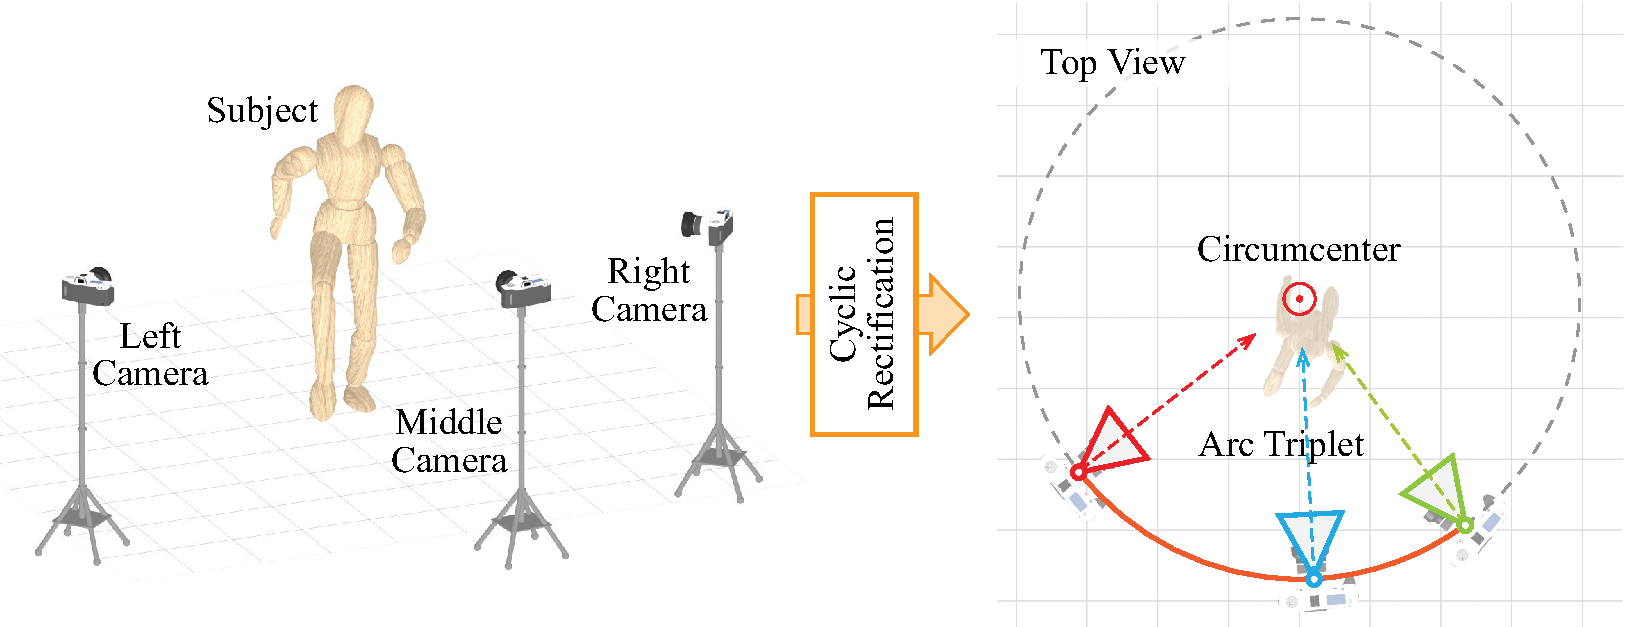
\includegraphics[width=\textwidth]{arc_triplets_rectification-eps-converted-to.pdf}
    \bicaption[环形校正示意图]{环形校正示意图。三个相机沿弧形分布。经过环形校正后,参考图像被对齐到一个公共圆上,即它们的光轴都通过其外心,这三张图被称为弧三元组。}[Cyclic rectification]{Cyclic rectification. Three cameras are configured along a circular path for capturing the reference images. After cyclic rectification, the reference images are aligned on a common circle (i.e., their optical principal axes all pass through the circumcenter) and they are called the arc triplet.}
    \label{fig:arc_rect}
\end{figure}

\subsection{拟合公共圆的外心}
现在考虑三个相机光心构成的三角形,其外心理论上是三条边的垂直平分线交点。由于这三个相机是在同一世界坐标系下进行标定的,外参中的向量$\{t_i | i=l, m, r\}$物理意义就是相机光心。因此$\{t_i - t_j | i, j = l, r, m; i \neq j\}$就是三角形边的向量表达。首先通过公式(\ref{eq:eq_1})求解线性方程组得到外接圆平面的法向$\mathbf{n}$。
\begin{equation} \label{eq:eq_1}
    \adddotsbeforeeqnnum%
    \mathbf{n} \cdot (t_i - t_j) = 0
\end{equation}
接下来按照公式(\ref{eq:eq_2})计算垂直平分线归一后的单位方向向量。
\begin{equation}\label{eq:eq_2}
    \adddotsbeforeeqnnum%
    \mathbf{d}_{ij} = \frac{\mathbf{n} \times (t_i - t_j)}{\|t_i - t_j\|}
\end{equation}
最后圆心$O$的求解通过对三条垂直平分线$\{\mathbf{d}_{ij}|i,j=l, m, r; i \neq j\}$做三角化求交点得到,如公式(\ref{eq:eq_3})。
\begin{equation}\label{eq:eq_3}
    \adddotsbeforeeqnnum%
    O = \frac{1}{2}(t_i + t_j) + \alpha_{ij}\mathbf{d}_{ij}
\end{equation}
其中$\{\alpha_{ij}|i,j=l, m, r; i\neq j\}$是各边中点沿着垂线方向追踪出去的长度,在方程中为未知数,数量为三。观察方程可知九个方程求解三个未知数,显然是一个超定线性系统,本文使用奇异值分解(SVD)求解。

\subsection{单应性变换}
本小节推导用来变换三张图像$\{\mathcal{I}_l, \mathcal{I}_r, \mathcal{I}_m\}$的单应性矩阵$\{\mathit{H}_i|i=l, r, m\}$,使得校正后的图像朝向上节推出的外心$O$。具体来说对相机的变换包括两步旋转:首先将相机的$y$轴与平面的法向$\mathbf{n}$对齐,然后将相机的$z$轴指向外心$O$。给定初始的相机的轴向$\{\mathbf{x}_i, \mathbf{y}_i, \mathbf{z}_i\} | i=l, r, m$,这里三根轴向量与标定的旋转矩阵满足关系$R_i = [\mathbf{x}_i, \mathbf{y}_i, \mathbf{z}_i]$,可以如公式(\ref{eq:eq_4})计算出相机的三根轴经过对齐后的新坐标轴。
\begin{equation} \label{eq:eq_4}
    \adddotsbeforeeqnnum%
    \begin{cases}
        \mathbf{x}_i' = \mathbf{y}_i' \times \mathbf{z}_i'\\
        \mathbf{y}_i' = \mathrm{sgn}(\mathbf{n} \cdot \mathbf{y}_i) \cdot \mathbf{n}\\
        \mathbf{z}_i' = \mathrm{sgn}(\mathbf{z}_i \cdot ({O} - t_i)) \cdot \pi(O - t_i)
    \end{cases}
\end{equation}
这里$i = l, m, r$,同样作用于弧上的全部三个相机。$\mathrm{sgn}(\cdot)$是符号函数,$\pi(\cdot)$表示向量做归一化函数。通过坐标轴与外参旋转矩阵的关系得到新的旋转矩阵为$R_i' = [\mathbf{x}_i', \mathbf{y}_i', \mathbf{z}_i']$。变换图像的单应性矩阵$\{H_i | i=l, r, m\}$可以用公式(\ref{eq:eq_5})计算。
\begin{equation}\label{eq:eq_5}
    \adddotsbeforeeqnnum%
    H_i = K_iR_i'^{\top}R_iK_i^{-1}
\end{equation}
而图像的变换通过计算变换前后的像素坐标关系可得。假设变换前的齐次像素坐标$\tilde{\mathbf{u}}=[u_x, u_y, 1]^{\top}$,则变换后的其次像素坐标$\tilde{\mathbf{u}}'=H_i \tilde{\mathbf{u}}$。在实际实现的时候通常需要通过反向计算,即从变换后的像素坐标位置计算对应到原图像中的像素坐标,以拷贝颜色值。


\section{视角变换网络}
本节介绍新设计的用于视角变换的卷积网络,它以经过环形校正后的三幅图像作为输入,合成一个在弧上均匀分布的图像序列,能够光滑连续地插值出原本弧两端相机之间的视角,本文给新设计的这个网络以英文缩写CVMN代替,网络的结构如图~\ref{fig:cvmn_pipeline}所示。
\begin{figure}[!htbp]
    \centering
    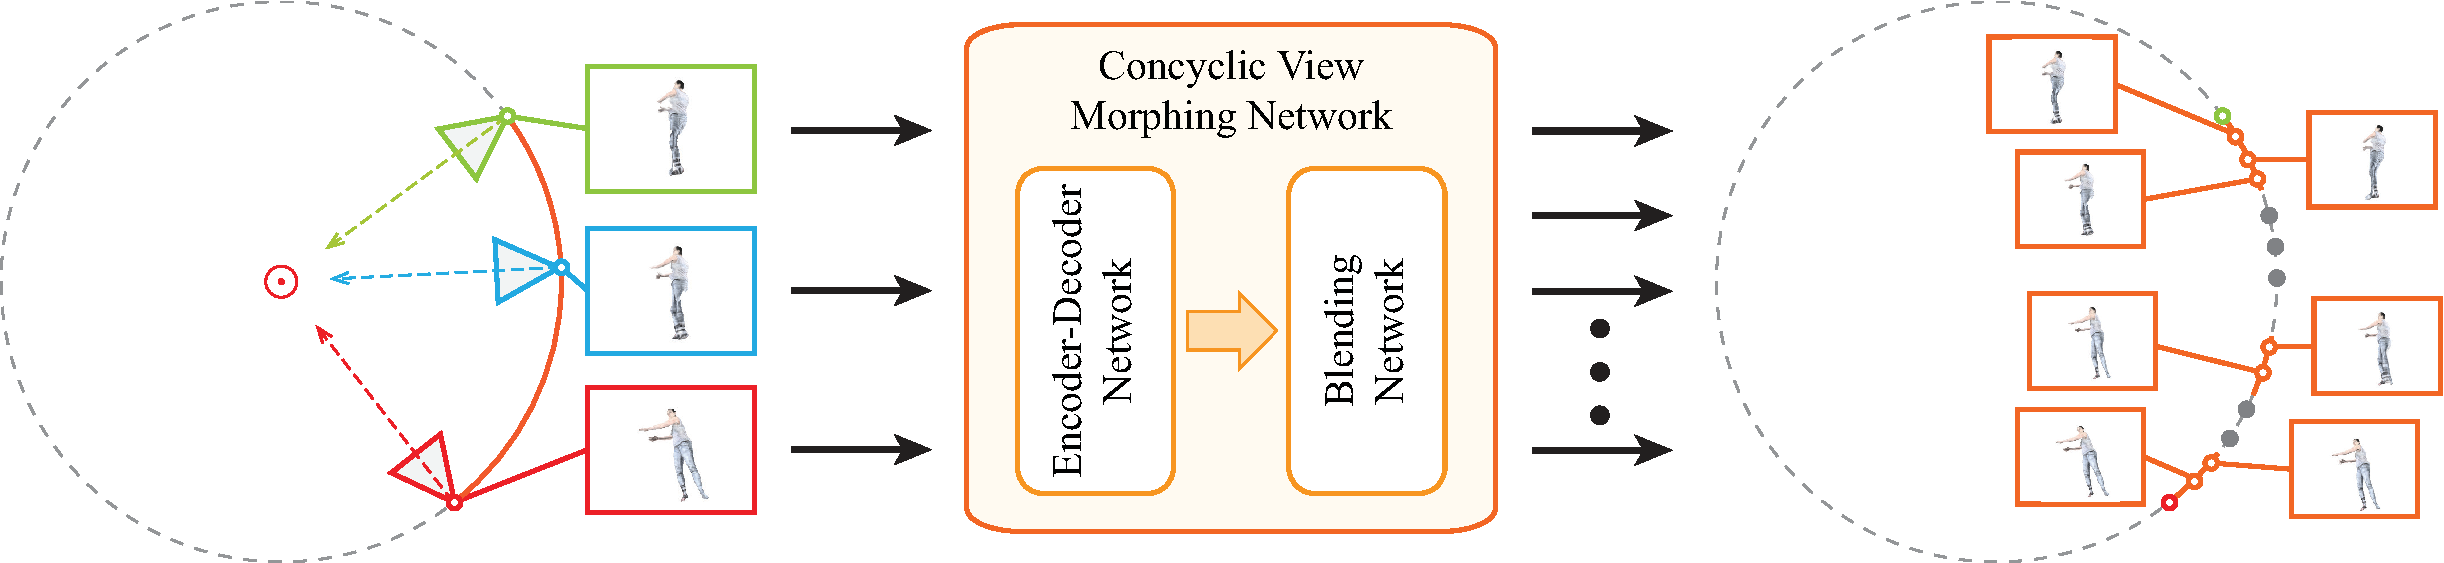
\includegraphics[width=\textwidth]{pipeline-eps-converted-to.pdf}
    \bicaption[视角插值网络整体结构图]{视角插值网络整体结构图。该网络以环形校正后的弧上三元组为输入并合成连续平滑的新视角序列。}[Overall structure of CVMN]{The overall structure of Concyclic View Morphing Network (CVMN). It takes the arc triplet as input and synthesize sequence of concyclic views.}
    \label{fig:cvmn_pipeline}
\end{figure}
本节中将从输入的三元组$\{\mathcal{I}_i | i=l, m, r\}$经过环形校正得到的弧上三元组记作$\{\mathcal{C}_i | i=l, m, r\}$。由于$\{\mathcal{C}_i\}$ 总可以被视为是严格分布在一段圆弧上的,CVMN可以看作是专门针对环形设定下的插值器。它包括两个子模块:一个是用于估计像素级运动场$\{\mathcal{F}_i | i=1, \dots, N\}$,也就是隐式几何的编码器---解码器网络,这个模块同时还会预测可见性蒙版$\{\mathcal{M}_i | i=1, \dots, N$,其中$N$代表生成的连续图片序列的数量;另一个模块是一个融合图像的生成模块,专门用$\{\mathcal{C}_i, \mathcal{F}_i, \mathcal{M}_i | i = l, m, r\}$来合成最终的视角序列。

\subsection{编码器---解码器网络}
编码器---解码器结构被证明在建立像素点匹配方面是很有效\citep{Ilg_2017_CVPR, newell2016},因此本节也采用这种结构来预测用于插值中间视图的像素级运动矢量场$\mathcal{F}_i$,同时指出这种表达与几何之间的关系。首先使用一个编码器来提取输出的三元组$\mathcal{C}_i$的相关特征,然后使用双分支的解码器来分别估计运动矢量场和可见性蒙版,总体结构如图~\ref{fig:cvmn_encoder_decoder}所示。
\begin{figure}[!htbp]
    \centering
    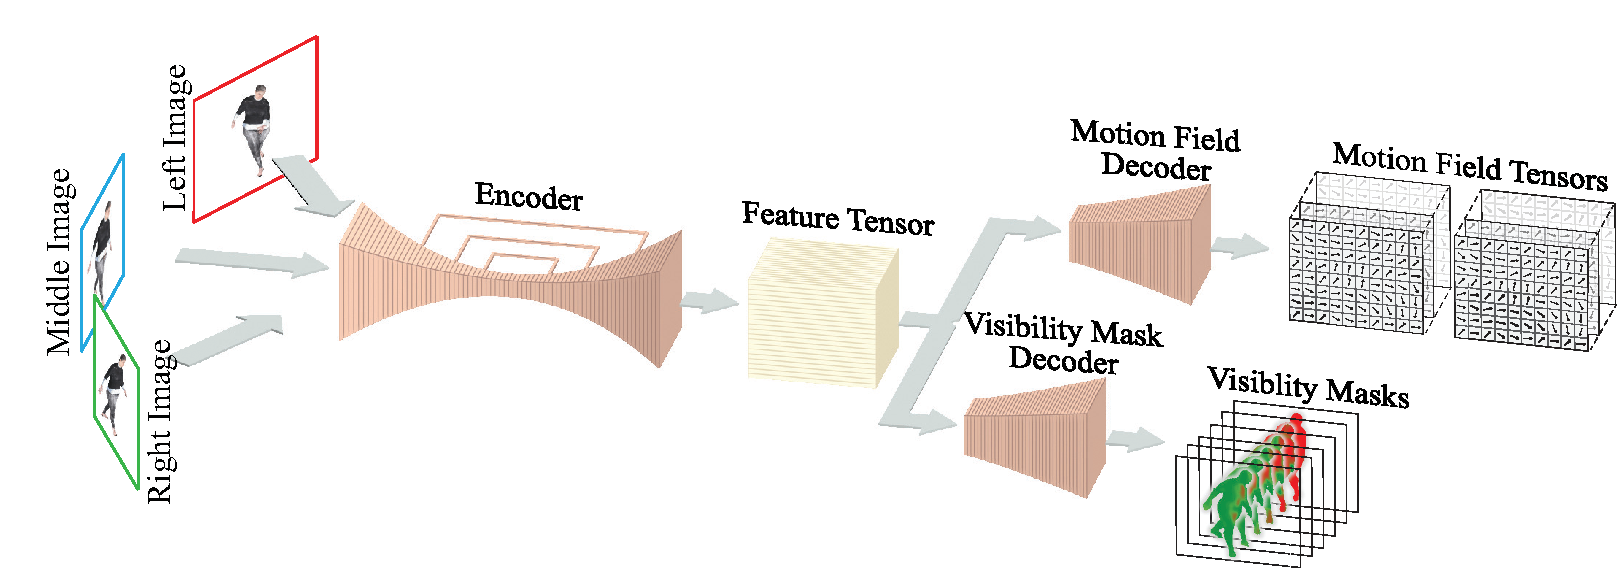
\includegraphics[width=\textwidth]{net_overview-eps-converted-to.pdf}
    \bicaption[编码器---解码器模块结构图]{编码器---解码器模块结构图。将输入的三元组进行特征编码并交给后续两分支解码器预测。}[The encoder-decoder network]{The encoder-decoder network. The encoder transfer the arc triplet to feature tensor and two decoders predict the motion field and visibility masks.}
    \label{fig:cvmn_encoder_decoder}
\end{figure}

编码器采用Hourglass结构\citep{newell2016}以便于捕捉不同尺度的特征。这种对称的先自下而上(从高分辨率到低分辨率)而后自顶而下(从低分辨率到高分辨率)的结构支持后续的解码器输出像素级别的预测,而这样的局部到全局的过程会重复若干层,最后输出与输入相同的全分辨率特征张量。由于输入含有三张图,编码器会对每张图单独编码后再把三张图得到的特征连接在一起。另一种考量是先将三张图像接在一起再一起编码,这样方案会由于图片通道数量上升而使编码器的参数数量暴涨,对于有限的计算量来讲是不切实际的。对于输入的三元组来说,实际上它们共用了一个仅对单张图片编码的编码器。

运动场解码器接收从编码器输出的特征,并预测输出序列中每一张图的像素偏移。具体来讲考虑了两个运动场:一个是针对三元组中的左图$\mathcal{C}_l$,另一个是针对三元组中的右图$\mathcal{C}_r$。运动场实际上存储的是每一对匹配像素之间的偏移向量,并且为了减少由于非均匀离散采样造成的空洞,采用了反向映射的方式来计算,即计算从待求图像$\mathcal{C}_i$到目标图像$\mathcal{C}_l$或$\mathcal{C}_r$的位移矢量。以$\mathcal{C}_l$为例,现在考虑要插值出一张中间图像$\mathcal{C}_i$。假设已知一对特征匹配,像素$p_l=(x_l, y_l)$在图$\mathcal{C}_l$,像素$p_i=(x_i, y_i)$在图$\mathcal{C}_i$中,则偏移向量$\Delta_i^l(p)=(u_i^l(p), v_i^l(p))$符合公式(\ref{eq:shift})描述的关系。
\begin{equation}\label{eq:shift}
    \adddotsbeforeeqnnum%
    p_l = p_i + \Delta_i^l(p)
\end{equation}
类似地可以计算出对右图$\mathcal{C}_r$的偏移向量$\{\Delta_i^r(p)=(u_i^r(p), v_i^r(p)) | p = 1, \dots, M\}$,这里$M$表示一张图上的所有像素个数。将对$\mathcal{C}_l$和$\mathcal{C}_r$的偏移向量连接起来,得到本节定义的4D运动向量$[u_i^l(p), v_i^l(p), u_i^r(p), v_i^r(p)]$。这个定义是针对$\mathcal{C}_i$的一个像素而言,如果将所有的像素放在一起,消去像素$p$后得到四个标量场$\mathcal{F}_i=(U_i^l, V_i^l, U_i^r, V_i^r)$,这里$U_i^l=\{u_i^l(p)|i=1,\dots,N, p=1, \dots, M \}$,其余三个标量场依从类似的构造。

在网络的结构上,反卷积层和卷积层交替排列来从特征张量解码出运动场。这种中间层设计的原因是由于实验表明在反卷积层后面加入适当的卷积层可以减少输出图像中的马赛克样块状瑕疵。由于运动场共包含$\{U_i^l, V_i^l, U_i^r, V_i^r\}$四个标量场,需要用四个解码器实例各自独立预测一个标量场,这是为了避免不同物理含义的标量场之间产生不应该的关联。值得注意的是,在预测运动场时是需要引入对应中间图像$\mathcal{C}_m$的特征张量的,尽管去掉它整个流程也能跑通,但后续的实验表明$\mathcal{C}_m$对于提高运动场估计的精度有很大帮助。

可见性蒙版解码器主要用来预测像素级的可见性信息。在视角改变较大的情况下,不同视角的遮挡变化会在视角变换中造成可见性的问题,待插值位置的像素很可能在不同图像中各有一部分可见。如果直接对输入视图根据运动场信息做插值并融合,会造成“鬼影”瑕疵,因此需要引入可见性蒙版来解决这个问题。给定一个待输出图像$\mathcal{C}_i$,定义两个可见性蒙版$\mathcal{M}_i^l$和$\mathcal{M}_i^r$,用来表示表示逐像素的可见性水平,这个可见性水平是相对输入图像$\mathcal{C}_l$和$\mathcal{C}_r$的。数值越大,说明在参考图像中看到这个像素的概率越高。在数值的范围上,$\mathcal{M}_i^l$和$\mathcal{M}_i^r$并不严格遵循概率取值必须在0到1之间的约束,而是可以取任意大于零的数值。实验表明这种放松有助于网络在训练中收敛地更快更稳定。

可见性蒙版解码器同样由交替的反卷积和卷积层构成,并以编码器输出的特征为输入,这点与运动场解码器类似。不同之处在于在输出层之前使用额外的ReLU层来约束输出值必须大于零。对于针对左右两个输入图的可见性蒙版$\mathcal{M}^l$和$\mathcal{M}^r$,分别各需要一个解码器实例进行预测。

\subsection{融合网络}
融合网络模块最终合成输出视图序列$\{\mathcal{C}_i|i=1, \dots, N\}$,用的信息包括左右两幅输入图像$\mathcal{C}_l$和$\mathcal{C}_r$和两个解码器的输出$\{\mathcal{F}_i|i=1,\dots,N\}$和$\{\mathcal{M}_i|i=1,\dots,N\}$,这里$N$表示输出的插值图像序列的帧数。融合网络模块的架构如图~\ref{fig:cvmn_blending}所示,
\begin{figure}[!htbp]
    \centering
    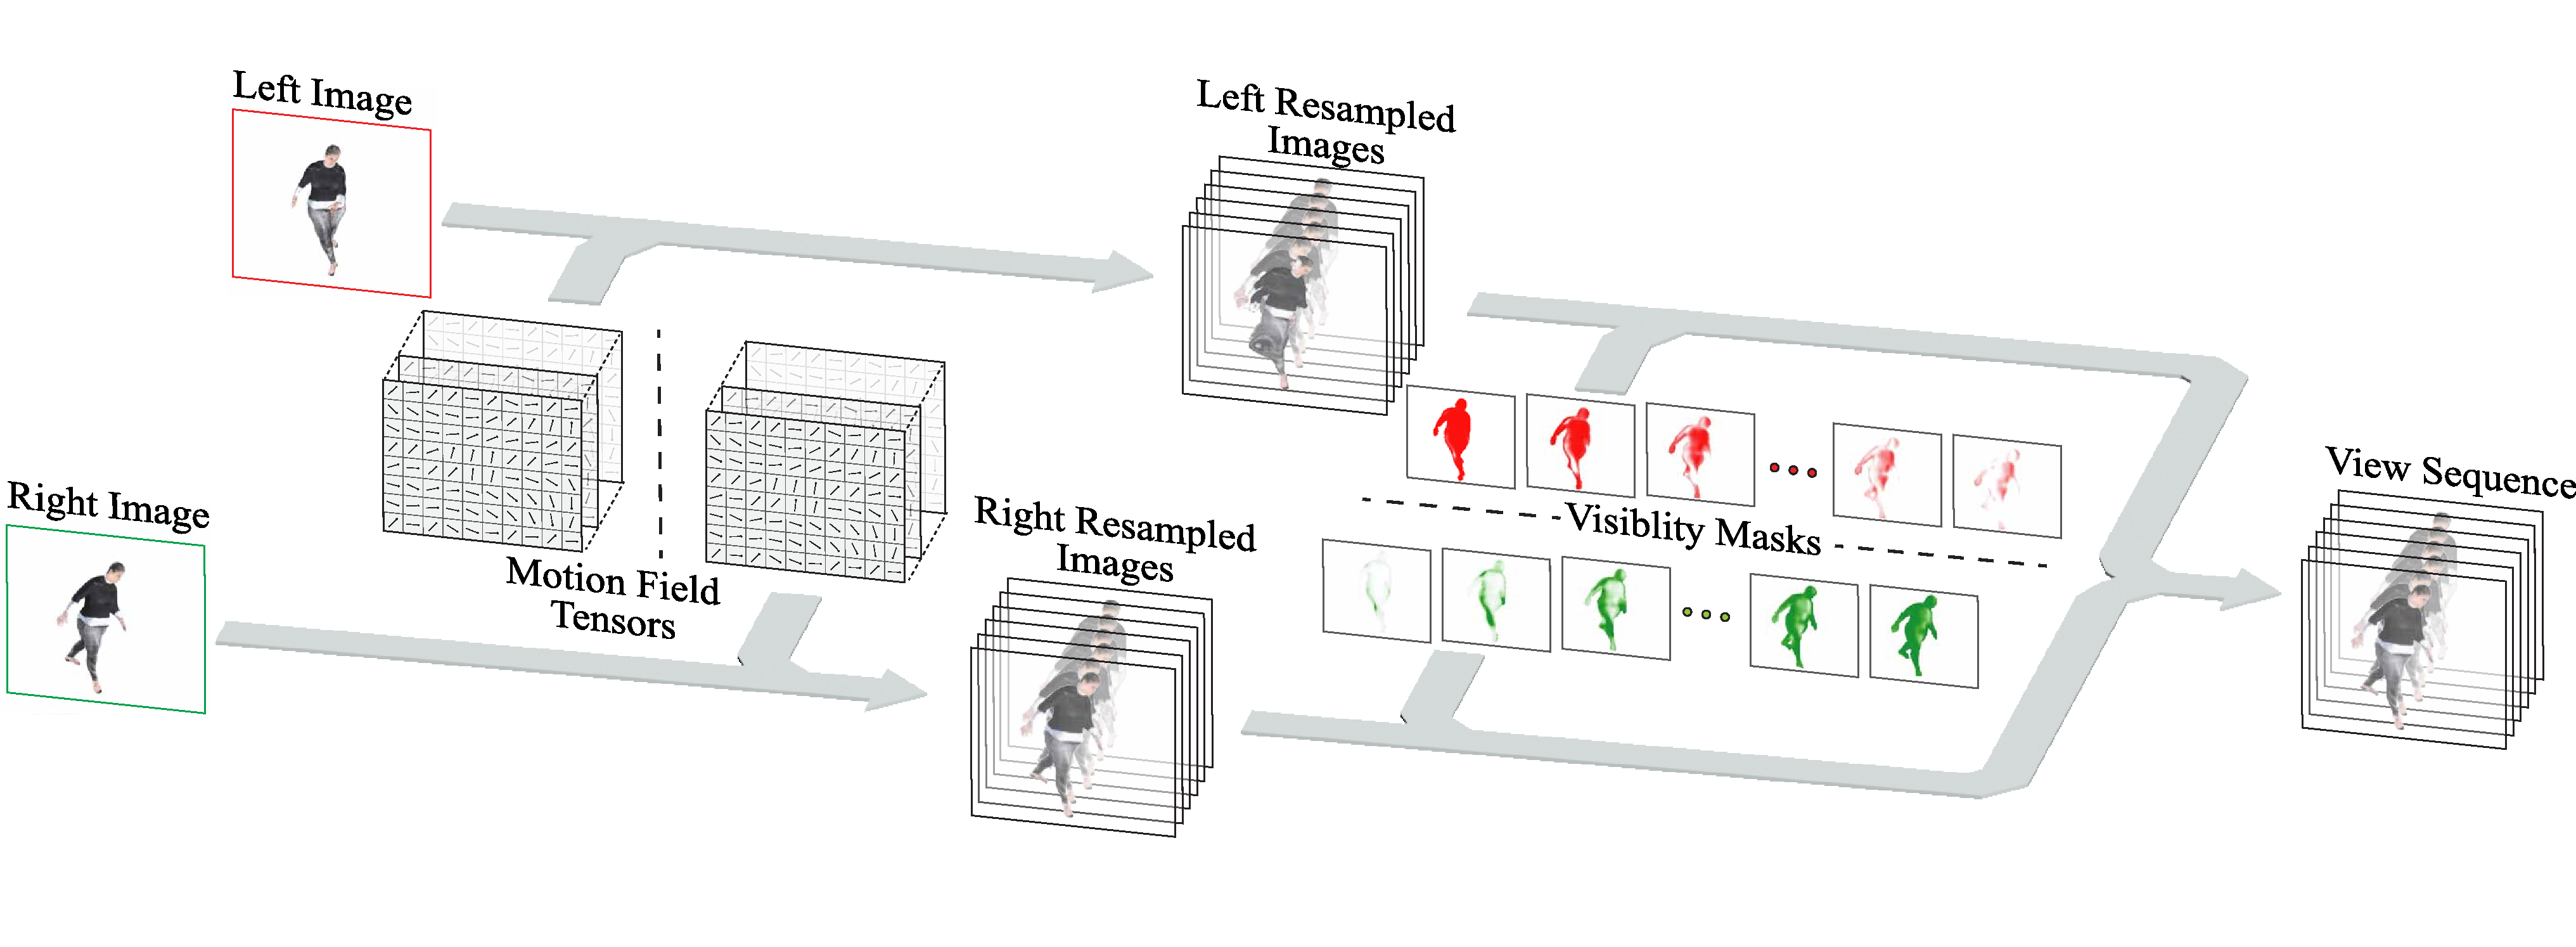
\includegraphics[width=\textwidth]{blending2.pdf}
    \bicaption[融合网络模块结构图]{融合网络模块结构图。利用预测的运动场信息和可见性蒙版信息合成插值帧序列。}[The blending network]{The blending network. Blending the morphed imaged using left reference image and right reference image, motion field and visibility masks.}
    \label{fig:cvmn_blending}
\end{figure}
首先由两个采样层对$\mathcal{C}_l$和$\mathcal{C}_r$进行重采样,重采样后的图像可以被公式$\mathcal{R}(\mathcal{C}_{\{l, r\}};U^{\{l, r\}}, V^{\{l, r\}})$表达,算子$\mathcal{R}(\cdot)$按照公式(\ref{eq:shift})对像素进行偏移量计算,对于每个新插值的视角,这会产生两幅重采样图像,一幅是从$\mathcal{C}_l$来的,一幅是从$\mathcal{C}_r$来的。接下来利用可见性蒙版$\mathcal{M}=(\mathcal{M}_l, \mathcal{M}_r)$作为权重,将重采样的图像加权融合。前面在描述可见性蒙版的时候提到解码器放松了蒙版的值域范围,因此这里需要做一步归一化操作,如公式(\ref{eq:eq_7})所示。
\begin{equation}\label{eq:eq_7}
    \adddotsbeforeeqnnum%
    \overline{\mathcal{M}}_i^{\{l, r\}} = \frac{\mathcal{M}_i^{\{l, r\}}}{\mathcal{M}_i^l + \mathcal{M}_i^r}
\end{equation}
这里的$i=1, \dots, N$。最终的合成图片序列可以通过公式(\ref{eq:eq_8})计算。
\begin{equation}\label{eq:eq_8}
    \adddotsbeforeeqnnum%
    \mathcal{C}_i = \mathcal{R}(\mathcal{C}_l; U_i^l, V_i^l) \otimes \overline{\mathcal{M}}_i^l + \mathcal{R}(\mathcal{C}_r; U_i^r, V_i^r) \otimes \overline{\mathcal{M}}_i^r
\end{equation}
运算$\otimes$代表逐像素的乘法。值得注意的是在整个融合模块里面所有的参数的运算都是固定的操作,没有任何可学习的参数,同时所有的计算都是连续可导的网络层,这意味着融合模块被链接进了整个神经网络且可以正常地进行反向传播操作。

\section{目标函数设计与隐式几何}
本节介绍网络训练的目标函数,为了引导CVMN的训练过程,设计目标函数的时候本方法考虑了三个方面的约束。第一个约束是合成的新视角的图片与真实值之间的相似度。由训练数据引入强约束,保证了能将数据集信息通过学习的方式融入网络参数,假设真实的监督视角图片记为$\{Y_i | i=1, \dots, N\}$,该约束直接比较图片之间的一范数,如公式(\ref{eq:eq_9})。
\begin{equation}\label{eq:eq_9}
    \adddotsbeforeeqnnum%
    \mathcal{L}_s = \sum_{i=1}^N \|Y_i - \mathcal{C}_i\|_1
\end{equation}
余下的两个约束均是从几何关系上推导出的,可以认为是不借助数据的自监督目标项,因此有必要先推导基于运动场与可见性的表达与三维几何的关系。以输入的左图$\mathcal{C}_l$为例,其内参矩阵$K_l$,外参旋转矩阵与光心坐标分别为$R_l$与$t_l$,待插值的图像$\mathcal{C}_i$,其内参矩阵$K_i$,外参旋转矩阵与光心坐标相应分别为$R_i$和$t_i$。现在考虑世界中的一点$P$,齐次像素坐标$\tilde{p_l}$和$\tilde{p_i}$分别表示在图中的位置,则满足公式(\ref{eq:epi})描述的关系。
\begin{equation} \label{eq:epi}
    \adddotsbeforeeqnnum%
    \begin{cases}
        P = R_l K_l^{-1}\tilde{p_l}d_l + t_l\\
        P = R_i K_i^{-1}\tilde{p_i}d_i + t_i
    \end{cases}
\end{equation}
其中$d_i$和$d_l$是点$P$在两个相机下各自的深度,而$p_i$实际上是由$p_l$和预测得到的运动场按照公式(\ref{eq:shift})描述。假设在上面式子里相机的内外参和像素坐标都是已知,那么将$P$、$d_i$和$d_l$视为未知数,整理两边可以得到六个线性方程,可以通过SVD分解快速求解出$d_i$和$d_l$。反过来如果知道$P$,则投影到两个相机的匹配像素点可以直接计算。

通过上面的论述明确了运动场计算出的偏移量作为隐式的几何表达,与直接给出3D点的位置在数学上是等价的。虽然计算3D点位置的计算复杂度相对更高,但这也是几乎所有隐式几何表达都有的一个特点。除此之外,当表达为偏移向量时,形式上可以将各个像素的偏移向量看作是以像素坐标为输入的二维函数,而这个函数显然是连续可导的,可以添加针对局部的光滑性约束。

现在介绍目标函数的第二个约束,该约束为从左右两个参考视图变换到当前图像时,来自左右的两幅变化图像之间的一致性。对于待插值出的每一辐图像$\mathcal{C}_i$,从左右参考图像$\mathcal{C}_l$和$\mathcal{C}_r$中各自能通过运动场变换出一张图像。尽管会出现遮挡变化,可是当注意力集中在可见区域时,在$\mathcal{C}_i$中某一像素,当其在左右图像中均为可见时候,这三个像素应该对应空间中同一个点,即从两边变换来的图像像素应该是基本一致的,由公式(\ref{eq:eq_11})表达。
\begin{equation} \label{eq:eq_11}
    \adddotsbeforeeqnnum%
    \mathcal{L}_u = \sum_{i=1}^N \|(\mathcal{R}_i^l - \mathcal{R}_i^r) \otimes \overline{\mathcal{M}}_i^l \otimes \overline{\mathcal{M}}_i^r \|_2^2
\end{equation}
这里使用两个可见性蒙版的乘法作为对可见性的置信近似,可以检验当某一像素对应的3D点在三张图中均为可见时,可见性权重相乘为1,而在其他情况下均小于1,且随可见性减小以二阶速度衰减到0。

第三个约束是运动场的估计应与参考图像之间满足对极几何约束,从公式(\ref{eq:epi})出发,消去$P$而仅关注$p_l$和$p_i$的关系如式(\ref{eq:eq_12})。
\begin{equation} \label{eq:eq_12}
    \adddotsbeforeeqnnum%
    R_l K_l^{-1}\tilde{p_l}d_l  =  R_i K_i^{-1}\tilde{p_i}d_i + (t_i - t_l)
\end{equation}
考虑同时在两边叉乘上$(t_i - t_l)$,为了表示叉乘,引入向量$t$对应的斜对称矩阵$\hat{t}$如公式(\ref{eq:eq_13})所示, 其中$t_1, t_2, t_3$表示三个分量,那么$t$叉乘上任意一个向量就等价于$\hat{t}$与该向量进行矩阵向量乘法。
\begin{equation} \label{eq:eq_13}
    \adddotsbeforeeqnnum%
    \hat{t} = \begin{bmatrix}
       0 & -t_3 & t_2  \\
       t_3 & 0  & -t_1 \\
       -t_2  & t_1 & 0
     \end{bmatrix}
\end{equation}
现在考虑公式(\ref{eq:eq_12})的两边同时叉乘上$(t_i - t_l)$,再将两边的$d_l$和$d_i$去掉,仅关注$p_l$与$p_i$之间的关系,则如公式(\ref{eq:eq_14})所示。
\begin{equation} \label{eq:eq_14}
    \adddotsbeforeeqnnum%
    (\hat{t_i} - \hat{t_l})R_l K_l^{-1}\tilde{p_l}  \sim  (\hat{t_i} - \hat{t_l})R_i K_i^{-1}\tilde{p_i}
\end{equation}
最后将偏移向量按照公式(\ref{eq:shift})代入,并观察公式(\ref{eq:eq_14})左边的向量按照数学定义应与$R_l K_l^{-1}\tilde{p_l}$垂直。以上分析都是以左图$\mathcal{C}_l$为例子,右图完全类似。由此此对极几何约束$\mathcal{L}_e$最终如公式(\ref{eq:eq_15})所示。
\begin{equation} \label{eq:eq_15}
\adddotsbeforeeqnnum%
    \begin{split}
        \mathcal{L}_e = \|\tilde{p_l}^\top K_l^{-\top} R_l^\top (\hat{t_i} - \hat{t_l})R_i K_i^{-1}(\tilde{p_l} + \tilde{\Delta}_i^l)\|^2 \\
       \qquad \qquad \qquad  + \|\tilde{p_r}^\top K_r^{-\top} R_r^\top (\hat{t_i} - \hat{t_r})R_i K_i^{-1}(\tilde{p_r} + \tilde{\Delta}_i^r)\|^2
    \end{split}
\end{equation}

将三个约束$\mathcal{L}_s$、$\mathcal{L}_u$和$\mathcal{L}_e$线性叠加起来就得到了如公式(\ref{eq:eq_16})所示的损失函数,其中$\lambda$和$\gamma$是平衡各个约束项的超参数。除开$\mathcal{L}_s$是直接衡量与真实数据的误差,其余两项分别是对运动场和可见性蒙版的约束,通过对设计的神经网络模块赋予物理和几何意义来强行使其在训练过程中满足相应的性质,以此达到将数据信息和先验知识结合的目的。
\begin{equation} \label{eq:eq_16}
\adddotsbeforeeqnnum%
        \mathcal{L} = \mathcal{L}_s + \lambda\mathcal{L}_u + \gamma\mathcal{L}_e 
\end{equation}

\section{本章小结}
本章介绍了结合深度学习和隐式几何表达的环形三相机视角变换插值的算法设计部分,包含新的三相机的环形校正算法和CVMN网络的整体结构。环形校正算法实际上将CVMN的输入统一变成了严格分布在圆弧上的三元组,缩小了网络需要处理的数据空间。CVMN网络又包括从图片中提取特征以及预测隐式几何表达的编解码器结构,以及无参数的且可导的融合生成模块。本章还介绍了针对CVMN的目标函数,能够同时被训练数据和隐式几何知识所约束,达到混合监督的目标。


\chapter{环形三相机视角插值实验及分析}\label{chap:CVM_experiment}

本章介绍CVMN的实验细节、实验结果分析以及同其他前沿方法的对比。为了说明本方法的优势,在仿真数据和真实数据上均进行了验证。仿真实验采用了SURREAL人体数据集\citep{varol2017}和ShapNet数据集\citep{shapenet2015}。本方法与相关的最新的视角合成方法DVM\citep{Ji_2017_CVPR},TVSN\citep{tvsn_cvpr2017}以及VSAF\citep{zhou2016view}进行了比较。实验证明本方法在视觉效果和定量指标方面都比这些方法要优。为了进行真实数据上的实验,搭建了一个实时的三相机采集系统,用来采集真实的3D人体动作,本方法在真实数据上生成了高质量的新视角合成效果。通过对整个环上的相机使用多次三相机的视角合成方法,本节最终成功展示针对人体的“子弹时间”效果。

\section{实验环境和设置}
本文用于实验的主机是64位x86架构机器,配备32GB内存和两块11GB显存的NVIDIA TITAN X显卡。
\begin{table}[!htbp] 
\bicaption[CVMN网络层的详细配置]{CVMN网络层的详细配置。表中包含了编码器、运动场解码器和可见性解码器。k/s/c分别代表卷积核/跨度/通道数。}[Configuration details for the encoder and decoder network]{Configuration details for the encoder and decoder network. k/s/c stand for kernel/stride/channel.}
\label{tab:cvmn_arch}
\centering
\footnotesize% fontsize
\setlength{\tabcolsep}{4pt}% column separation
\renewcommand{\arraystretch}{0.9}%row space 
\begin{tabular}{l c l ccc  l ccc}
\hline
\multicolumn{2}{c}{Encoder} & \multicolumn{4}{c}{Motion Field Decoder} & \multicolumn{4}{c}{Visibility Mask Decoder} \\
\hline
\multicolumn{2}{c}{hourglass} & Type & k & s & c  & Type & k & s & c \\
\hline
stack       & 1   & Input  & - & - & 144 & Input   & - & - & 144 \\
block       & 2   & Conv   & 7 & 1 & 288 & Conv    & 7 & 1 & 288 \\
feature     & 104 & MaxPool& 3 & 2 & 288 & Conv    & 3 & 1 & 576 \\
inplanes    & 18  & Conv   & 3 & 1 & 576 & Conv    & 1 & 1 & 576 \\
out channel & 48  & Conv   & 1 & 1 & 576 & DeConv  & 3 & 1 & 288 \\
            &     & DeConv & 4 & 2 & 288 & DeConv  & 3 & 1 & 144 \\
            &     & DeConv & 3 & 1 & 144 & Conv    & 3 & 1 & 144 \\
            &     & Conv   & 1 & 1 & 144 & Deconv  & 3 & 1 & 24 \\
            &     & DeConv & 3 & 1 & 24 & Conv   & 1 & 1 & 24 \\
            &     & Conv   & 1 & 1 & 24 & ReLU    & - & - & 24 \\
            &     & Conv   & 1 & 1 & 24 &   &  &  &  \\
\hline
\end{tabular}
\end{table}
为了训练CVMN使用了Adam算法,其中的两个参数$\beta_1=0.9$,$\beta_2=0.999$,初始的学习率为$0.0001$。单次进行训练时仅使用单块显卡,单个batch的大小为8。本方法评估的图片分辨率上至256。表~\ref{tab:cvmn_arch}展示了CVMN的网络层详细参数,包括编码器的模块参数以及运动场编码器和可见性编码器的网络层结构和数据维度。CVMN的输入为经过环形校正后的图片三元组,编码器对每张图单独编码为48通道的张量,再把三张图的特征连接在一起组成144通道张量,继续喂给解码器做后续的预测。

\section{人体数据集实验}
\subsection{数据准备}
SURREAL\citep{varol2017}数据集包含了大量的由SMPL\citep{loper2015smpl}参数化的人体运动序列。每个运动序列都包含连续的运动过程。为了生成不同场景的训练和测试数据,首先从数据集里挑选出三维任何模型和纹理,最终从312个序列中导出了30439个人体模型,以及929张不同的纹理,每个模型的纹理是随机指定的。这些带纹理贴图的模型通过渲染生成训练集和测试集的数据。具体来说,虚拟相机在一个环上移动并始终保持相机光心对准圆心,这符合环形校正后的图片分布规律。对于一个序列,渲染算法选取30个不同的球坐标纬度,每个纬度渲染24张图片作为一组,这一组图片的最大视角变化范围随机在30度到120度中选取。总共渲染得到超过100万组序列,每一个24张图片的序列为一组数据,测试集由这超过100万组的十分之一构成,其余用于训练。

在每一轮训练过程中,这些序列的迭代顺序是随机的。给定一个序列$\mathcal{S}=\{\mathcal{C}_1, \mathcal{C}_2, \dots, \mathcal{C}_{24}\}$,需要生成弧上的三元组。生成算法总是将$\mathcal{C}_1$作为最左边的$\mathcal{C}_l$了,同时将$\mathcal{C}_{24}$作为最右边的$\mathcal{C}_r$。中间的$\mathcal{C}_m$从$\mathcal{S}$中的选择概率服从高斯分布,这样的随机性能够迫使CVMN对相机位置的变化有一定的容忍度。在实际情况下,三个相机一般不会刚好完美分布在外接圆上均匀的位置,同时中间的相机一般也不太可能过于接近两边的相机。图~\ref{fig:cvmn_surreal}展示了两个通过CVMN合成的新视角的部分图片。三个输入的参考视图使用框来标记,可以看到形状和纹理在生成的视图中保持得很好。
\begin{figure}[!htbp]
    \centering
    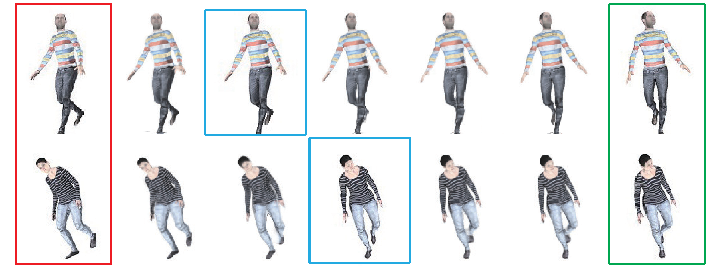
\includegraphics[width=\textwidth]{surreal_sequence-eps-converted-to.pdf}
    \bicaption[CVMN合成的人体数据示例]{CVMN合成的人体数据示例。由于空间限制,图中仅展示24张生成的图片序列中的7张,其中带框的是输入图片。}{Morphing sequences synthesized by CVMN. Seven samples are picked from the whole sequence (24 images in total). The boxed images are the input reference views.}
    \label{fig:cvmn_surreal}
\end{figure}

\subsection{模型的简化对比实验}
为了说明CVMN在设计上的优势,以及弄清楚每一个模块的必要性,首先把CVMN与另外的两个自身变体进行对比。第一个变体代号CVMN-I2,它仅仅使用$\mathcal{C}_l$和$\mathcal{C}_r$两张图片作为编码器的输入;第二个边体代号CVMN-O3,它则是在解码器中对全部的三张图片预测运动场$\mathcal{F}$和可见性蒙版$\mathcal{M}$,同时在融合生成模块中也使用全部三张图像。网络的训练参数全部保持一致。可以发现,这两个变体主要针对编码器和解码器模块到底需要几张图进行了探索。公式(\ref{eq:eq_16})中对应的损失函数超参数$\lambda$和$\gamma$为别设置为10和1,并在所有的训练数据中保持不变。在比较生成的插值图片序列和真实值的差异时,用平均绝对误差(MAE)和结构相似指数(SSIM)这两个指标来度量。

\begin{table}[!htbp]
\bicaption[SURREAL数据集上的定量指标结果]{SURREAL数据集上的定量指标数据。}{Quantitative evaluation on the SURREAL dataset.}
\label{tab:cvmn_surreal}
\centering
\footnotesize% fontsize
\setlength{\tabcolsep}{4pt}% column separation
\renewcommand{\arraystretch}{0.9}%row space 
\begin{tabular}{c cccc}
\hline\noalign{\smallskip}
Architecture & CVMN & CVMN-I2 & CVMN-O3 & DVM\citep{Ji_2017_CVPR} \\
\noalign{\smallskip}
\hline
\noalign{\smallskip}
MAE  & \textbf{1.453} & 2.039 & 2.175 & 3.315\\
SSIM & \textbf{0.983} & 0.966 & 0.967 & 0.945\\
\hline
\end{tabular}
\end{table}
表~\ref{tab:cvmn_surreal}展示了CVMN与两种变体的结果对比,CVMN的结果明显优于两种变体。这是因为中间视图$\mathcal{C}_m$提供了更好的遮挡信息,使得编码器能提取出额外的信息。图~\ref{fig:cvmn_i2_o3}展示了CVMN和两种变体的插值结果对比。
\begin{figure}[!htbp]
    \centering
    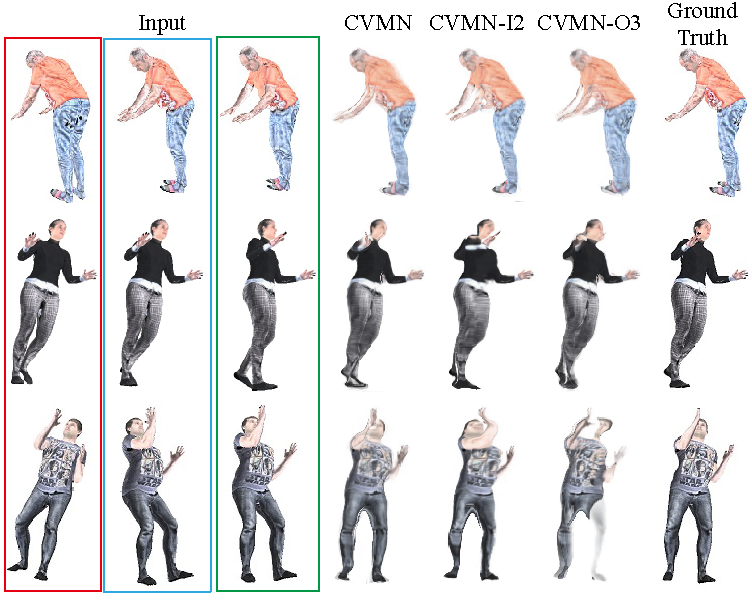
\includegraphics[width=\textwidth]{supplemental_surreal_I2_O3.pdf}
    \bicaption[CVMN与变体的对比结果图]{CVMN与变体的对比结果图。从左到右分别是:三个视角的输入参考图片,CVMN输出的结果,CVMN-I2输出的结果和CVMN-O3的输出结果。}{Qualitative comparison results for the ablation study. From left to right: the three input reference images, sample synthesized image by CVMN, CVMN-I2, and CVMN-O3, and the ground truth view.}
    \label{fig:cvmn_i2_o3}
\end{figure}
比较这些结果可以发现CVMN的瑕疵更少,与真实参考图片更接近。另外两个变体在发生遮挡变化的区域附近则出现了明显的瑕疵,直接说明了编码器提取特征过程中中间图像的巨大作用,以及解码过程中中间图像应该去掉,否则会将合成过程变得更加复杂而具有歧义。

\subsection{CVMN与DVM的比较}
DVM\citep{Ji_2017_CVPR}同样是利用深度学习求解视角插值的最新方法,由于原作者并未开源代码,实验中是按照原论文的描述复现了算法。考虑到DVM仅能插值两张图片正中间的视角,在SURREAL数据集上进行对比时,从$\mathcal{S}=\{\mathcal{C}_1, \mathcal{C}_2, \dots, \mathcal{C}_{24}\}$中随机选取一对图片$(\mathcal{C}_a, \mathcal{C}_b)$作为DVM的输入,同时选择$\mathcal{C}_{\lfloor (a+b)/2\rfloor}$作为监督数据。定量数据结果如表~\ref{tab:cvmn_surreal}最后一列所示,图~\ref{fig:cvmn_dvm}展示了出了部分插值出的新视角结果,本方法的效果明显优于DVM。从图中可以看出,DVM合成的图像重影和模糊现象比较严重,这是由于DVM无法应对大视角范围下的复杂遮挡变化问题,这在图中人物手臂的部分尤为明显。
\begin{figure}[!htbp]
    \centering
    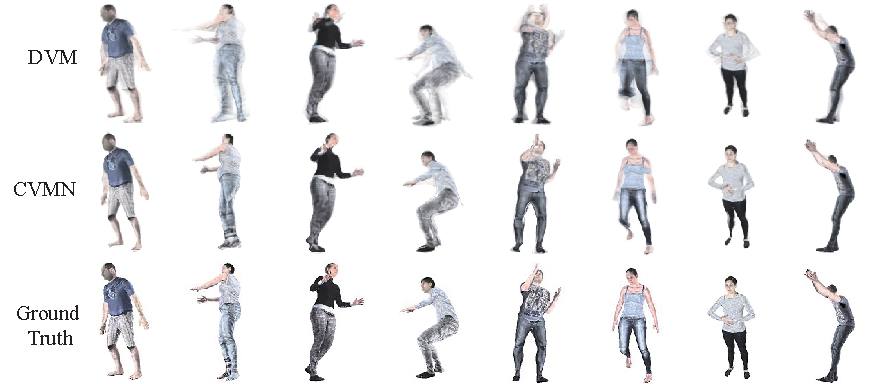
\includegraphics[width=\textwidth]{surreal_compare_DVM_1.pdf}
    \bicaption[与DVM比较的结果图]{与DVM比较的结果图。CVMN的输出图片中选取了中间的视角与DVM比较。}{Comparison with DVM. The middle view is picked in the synthesized sequence from CVMN to compare with DVM.}
    \label{fig:cvmn_dvm}
\end{figure}

\section{ShapeNet数据集实验}
为了进一步说明本方法的通用性,本节介绍在ShapeNet数据集\citep{shapenet2015}上的实验结果,以证明本方法对基本任意类型的3D对象都能表现很好。具体来说,本实验从整个ShapeNet数据集中挑选出汽车和椅子模型进行测试。数据的准备过程类似于之前对SURREAL所作的操作。视角变化的范围设定在30度到90度之间。用于测试的数据量为百分之二十,其余数据用于训练。用于训练的数据组数对于汽车模型和椅子模型分别是约10万组和20万组。训练过程与SURREAL设置一致。

在ShapeNet数据集上,本方法与包括DVM\citep{Ji_2017_CVPR},TVSN\citep{tvsn_cvpr2017}以及VSAF\citep{zhou2016view}在内的三个最新方法进行了定性和定量的比较实验。对于VSAF和TVSN,本实验采取了原作者提供的预训练模型。在渲染它们的测试数据时,插值视角范围从$\{40^\circ, 60^\circ, 80^\circ\}$中选取,使得测试角度在真实图片中有精确对应,从而保证比较的公平性。本实验使用MAE作为误差度量,实验数据结果如表~\ref{tab:cvmn_shapenet}所示。
\begin{table}
\bicaption[ShapeNet数据集上的定量指标数据]{ShapeNet数据集上的定量指标数据。}[Quantitative evaluation on the ShapeNet dataset]{Quantitative evaluation on the ShapeNet dataset.}
\label{tab:cvmn_shapenet}
\centering
\footnotesize% fontsize
\setlength{\tabcolsep}{4pt}% column separation
\renewcommand{\arraystretch}{0.9}%row space 
\begin{tabular}{c c c c c}
\hline\noalign{\smallskip}
Method  & DVM\citep{Ji_2017_CVPR} & VSAF\citep{zhou2016view} & TVSN\citep{tvsn_cvpr2017}& CVMN \\
\noalign{\smallskip}
\hline
\noalign{\smallskip}
Car   & 3.441 & 7.828 & 5.380 & \textbf{1.608}\\
Chair & 5.579 & 20.54 & 10.02 & \textbf{2.777}\\
\hline
\end{tabular}
\end{table}
部分可视化对比结果如图~\ref{fig:cvmn_shapenet}所示。TVSN在椅子数据上的结果表现比较差,而DVM仍然有明显的重影瑕疵。VSAF的可视化效果比其他方法差得较多,没有在图中展示。本方法在椅子和汽车类别下均能较好地合成新视角,生成的插值图像能够较好地接近真实数据。
\begin{figure}[!htbp]
    \centering
    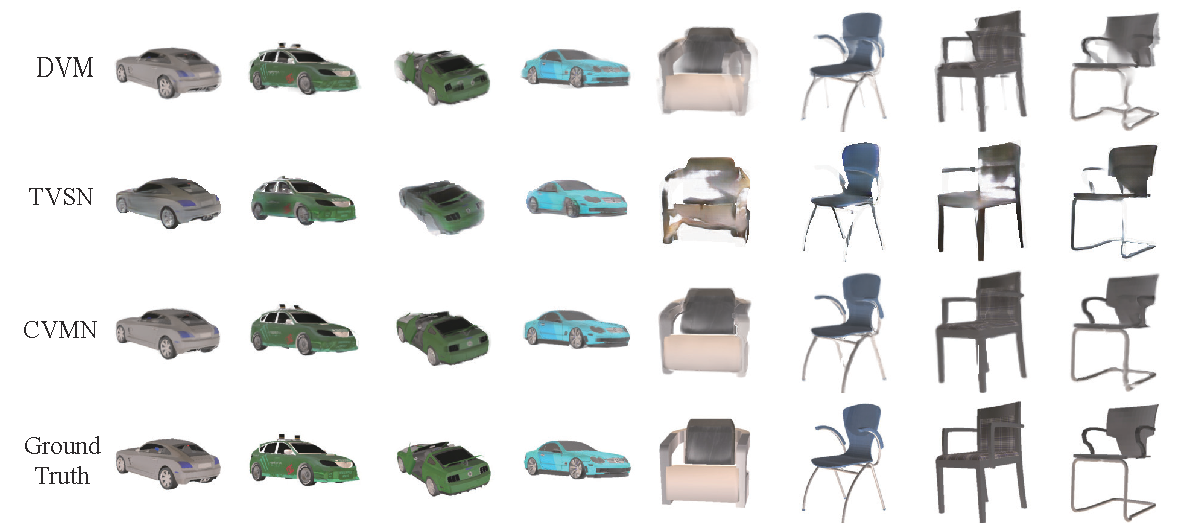
\includegraphics[width=\textwidth]{shapenet_result_1.pdf}
    \bicaption[ShapeNet数据集上的可视化结果对比图]{ShapeNet数据集上的可视化结果对比图。}{Quanlitative comparisons with DVM and TVSN on ShapeNet.}
    \label{fig:cvmn_shapenet}
\end{figure}

\section{真实场景实验}
本节介绍真实场景下的动作序列实验。用来采集真实数据的采集系统是一个专门搭建的三摄像机系统。所使用的工业相机使用网线连接到一台采集服务器,同时使用硬件触发进行同步。相机围绕拍摄对象距离约3米左右,三个相机使用多视角视图配准(SfM)进行标定。为了测试不同视角范围下的输入,捕捉不同序列的时候相机的位置进行了移动。总的来说,左右摄像机之间的视角变换在30度到60度之间。

对采集得到的图像,首先进行预处理,利用预先标定的内参去除相机畸变,并使用背景减除算法移除背景。然后利用环形校正或者对齐到圆环上的三元组。最终,将弧三元组喂给CVMN网络来合成新的视角序列。由于缺乏真实标注数据用于监督训练,本实验中的网络参数使用的是在SURREAL数据集\cite{varol2017}上训练的结果。图~\ref{fig:cvmn_real}展示了合成结果。尽管真实数据由于噪声、高动态范围和光照的剧烈变化而更具挑战性,但是在仿真数据集上训练出的网络参数依然可以产生高质量的合成插值结果。这表面本方法的准确性和健壮性都很好。图中也与DVM的结果进行了对比,其重影瑕疵由于大视角的变化,依然很明显。
\begin{figure}[!htbp]
    \centering
    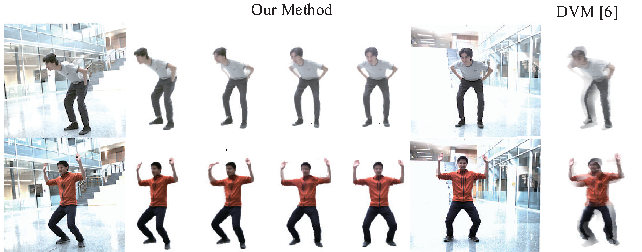
\includegraphics[width=\textwidth]{real_scene_qualitative-eps-converted-to.pdf}
    \bicaption[ShapeNet数据集上的可视化结果对比图]{真实数据结果图。挑出了合成序列中的四张展示出来。DVM合成的中间视角显示在最右边一列。}{Real scene results. Four samples from the morphing sequence. The middle view synthesized by DVM is shown on the right column.}
    \label{fig:cvmn_real}
\end{figure}

\section{子弹时间效果的渲染结果}
本节介绍利用提出的环形视角变换方法实现“子弹时间”效果的实验。由于合成的图片序列是已经对齐到一个理想圆环上的,所以本身非常适合通过多次变换相邻的视图三元组,来创建子弹时间。本实验仍然在SURREAL数据集上完成,从围绕一个对象拍摄一圈的相机角度中选出6组环上的图片三元组,实验中规定相邻的两组三元组会共享一张图,总计就是12张图。对每一组环上的三元组,利用本方法生成变换序列,然后连接在一起,就构成了完整的一整圈视角。图~\ref{fig:bullet_time}展示了部分实例图像。
\begin{figure}[!htbp]
    \centering
    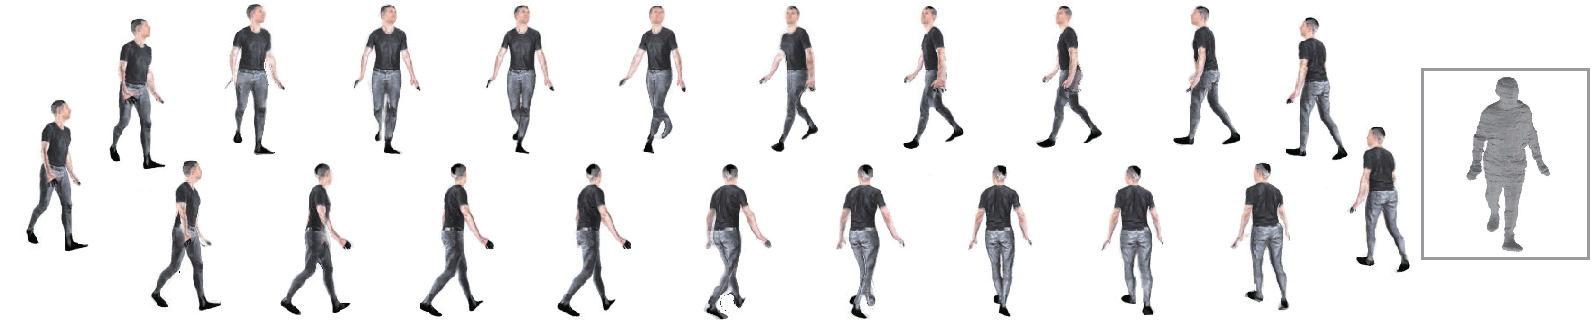
\includegraphics[width=\textwidth]{bullet_time-eps-converted-to.pdf}
    \bicaption[子弹时间效果渲染图]{子弹时间效果渲染图。图中展示了144个渲染视角中的21个,图的右边显示Visual hull 得到的几何模型效果。}{Bullet-time effect rendering result. Showing 21 samples out of the the 144 views in the bullet-time rendering sequence. Visual hull reconstruction from the view sequence is shown on the right.}
    \label{fig:bullet_time}
\end{figure}

图的右边同时展示了用全部的插值图像的轮廓信息计算出的人的三维模型。观察模型可以发现,人的大致几何是能够恢复出来,但是包括面部、手脚和身上衣服的纹理细节是缺失的。在本文算法的章节中提到了CVMN中用来表示隐式几何的运动偏移向量场和可见性蒙版,这里恢复出的几何正好印证了渲染图片质量与隐式几何表达之间的联系。在渲染任务中,关注的重点在于渲染结果而不是几何,本实验部分地论证了渲染结果的提升不一定要完全依赖精确的几何,即粗略的几何模型很可能已经满足渲染需求,但同时几何表达对于图片信息的融合也不可或缺,毕竟在本实验中仅仅对图片进行监督实际上足以得到大致准确的几何模型。

\section{本章小结}
本章介绍了环形视角变换方法在多个数据集上的实验结果。通过在仿真的人体和一般物体的数据上测试,说明了提出的方法具有普适性。通过在真实数据上的测试,说明了提出的方法具有泛化性和鲁棒性,尤其是CVMN网络模块的设计遵循奥卡姆剃刀原则。在与其他的视角变换及合成算法的对比中,效果超越了其他方法。最后展示了“子弹时间”效果以及利用合成的新图片反过来重建出了几何模型,说明了隐式几何表达在本方法中的必要性,同时讨论了几何先验在渲染任务中既不可或缺又可一定程度上折衷的辩证思想。


\chapter{多视角投影结合隐函数的点云重建方法}
从点云数据重建出完整的表面是许多几何相关应用的关键步骤,例如虚拟换装,自由视角渲染等。随着扫描设备的普及,从专业的3D扫描仪到消费级深度传感器如微软的Kinect,再到如今最新的手机上的深度摄像头,获取点云的途径变得多样。正因如此,点云的质量水平也随着设备不同而差异巨大,反观点云重建的算法能达到的效果仍然有提高空间。原始点云的随机噪声、非均匀采样以及遮挡空洞等问题,都是重建算法应该解决的问题。根据是否基于数据驱动提取先验知识,可以将点云重建的已有研究工作分为两类。

\citet{berger17}撰写了关于传统点云重建的详尽综述,根据假设的不同、噪声的种类以及输出的表达形式对方法进行了分类与比较。\citet{digne11}通过连续迭代曲率的方法对点云进行平滑操作并三角化,\citet{OHRHALLINGER2013645}通过优化三角面片的最长边之和来求解稀疏点云的表面,然而这些方法对噪声十分敏感。除了这类组合优化的思路,另一类方法从一个初始的参数化模板开始变形,逐渐逼近点云数据。\citet{sharf06}以单位球为起点将其置于点云的内部,一边变形一边细分,以此渐进拟合到点云。\citet{li10}用一维的骨骼参数化模型拟合线状结构,来处理比较细的结构。这类方法往往受到模板的限制,无法改变拓扑结构,当点云的拓扑与模板有明显差异时,拟合结果较差。为了对抗噪声同时能够处理任意的拓扑关系,许多方法用隐函数来表达几何,通过拟合点云求解出隐函数,最后从中提取水平集(Level set)作为表面。\citet{hoppe92}首次引入了这套方法,隐函数作为几何表达形式的想法开始受到广泛关注,探讨隐函数本身表达的方法开始出现,包括频域上的傅里叶系数\citet{kazhdan05}和小波变换\citet{manson08},\citet{ohtake05}在多尺度的层级模型下利用径向基函数(RBF,radial basis functions),提高了非均匀采样情形下的重建效果。\citet{alliez07}利用点云的维诺图(voronoi diagram)和主成分分析(PCA)来对隐函数梯度进行建模,通过求解系统的特征值(SVD)对隐函数进行拟合。而在以隐函数为基础的这类方法中,泊松重建\citep{kazhdan2013, kazhdan2006}具有绝对的优势。它以点云的位置信息和法向信息作为输入,约束重建后的表面要逼近点云,同时表面的法向与点云的法向保持一致。但由于所有的分析仅基于输入数据本身,没有任何额外先验,重建出的表面往往过于平滑且缺少细节,针对噪声和空洞的补全往往是不正确的。更糟糕的是,大多数情况下输入点云的法向需要从点云本身去计算,这个过程本身对噪声和采样密度就十分敏感,这无疑放大了噪声的影响从而大大限制了重建出的几何质量。

最近,数据驱动的点云重建方法有了进展,这些方法试图从一定规模的数据集中学到集合的先验。\citet{ladicky17}使用回归森林(regression forest)来从点云数据预测空间任意点到表面的距离(SDF,signed distance function),并使用八叉树和GPU加速。后来的方法倾向于用一个全局特征向量来表达整个几何,一般使用神经网络编码器从点云数据中获得。对于给定的数据集,特征向量一般在高维空间中存在结构化的分布,因此网络从中学到的信息就可以用来作为一类几何的先验。隐函数在空间离散后形成三维网格,一般为固定分辨率,隐函数的值存储在各个格点上。\citet{ogn2017}用八叉树来减少离散网格的存储开销,仅仅子啊叶子节点上使用卷积网络进行隐函数的预测。\citet{groueix2018}以固定分辨率的二维平面作为参数化模板,使用多歌不同参数的模板单体一起来拼成整个表面,具有较好的泛化性能。最新的工作抛弃了空间离散化的形式,转而使用神经网络来直接表达连续的隐函数\citep{chen19, meshcheder2019cvpr, park2019cvpr},将空间中的任意点映射成隐函数值,这样的表达不再受到离散网格的分辨率影响,适合表达具有复杂拓扑结构的表面,理论上能够取得任意的精度。

本章的点云重建方法在此基础上,取隐函数为几何表达形式,结合新的点云编码方法进行点云重建。对于带噪声和非均匀采样的点云,甚至是由于遮挡造成空洞的人体扫描点云,新方法都能重建出细节丰富的完整模型,保留诸如衣服褶皱等几何细节,同时能正确处理不同拓扑的情况。新方法的核心思想在于对点云的结构化处理,先将点云渲染到多个视角得到深度图,再用编码器将点云图映射到特征空间。隐函数由多层感知机(MLP,multilayer perceptron)实现,对于空间中任意点,通过投影到各个视角上取得点云的特征,经过融合后由隐函数映射成表达该点位于几何内部还是外部的概率,整体算法框架如图\ref{fig:pc_pipeline}所示。
\begin{figure}[!htbp]
    \centering
    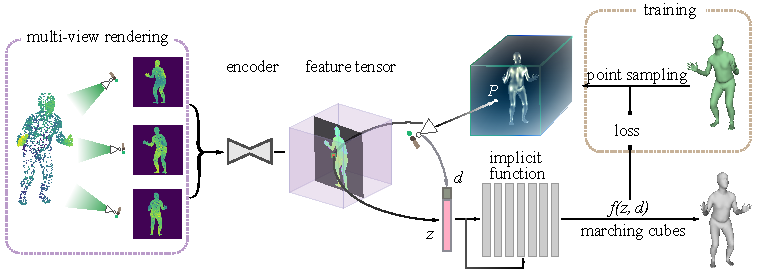
\includegraphics[width=\textwidth]{pipeline_pc.pdf}
    \bicaption[算法框架图]{算法框架图。对于输入点云,经过多视角投影和特征提取后,给定空间点$P$,投影到各个视角中得到特征向量$z$,连同投影得到的深度$d$,经过隐函数得到位于表面几何内/外部的概率$f(z, d)$,提取等值面后得到输出三角面片。}[Pipeline of pointcloud reconstruction]{Pipeline of pointcloud reconstruction. After multi-view projection and feature extraction, a 3D point $P$ is projected to each view to get the feature vector $z$ and the depth $d$, the implicit function predicts the inside/outside probability. The surface is extracted using marching cubes.}
    \label{fig:pc_pipeline}
\end{figure}
相比于直接用三维网格对点云进行光栅化,通过投影到二维网格的方式更加节省内存。借助基于卷积操作的特征提取过程,可以在多个尺度上对点云进行去噪和空洞补全。通过在两个人体数据集上的实验,新方法可以生成更加精确和富有细节的点云重建结果。主要的贡献包括:提出了结合隐函数与数据驱动的点云重建算法。利用端到端的可导过程表达点云到表面几何的生成,能从已有的数据中学习处理点云噪声和空洞的知识,提升点云重建的质量和鲁棒性;结合可渲染和基于卷积的编码器对点云作结构化处理,节省内存地同时对点云进行了去噪和补洞操作,同时新算法能够处理任意数量的视角,可扩展性极强。

\section{隐函数的几何建模过程}
将真实的几何表面记作$M$,点云数据$P=\{p_1, \dots, p_N\}$从其上采样得到,采样过程中设备噪声会叠加到点云的位置上,视角变化和自遮挡也会造成空洞。$M$可以表达为函数$F(\cdot)$的等值面,如公式(\ref{eq:pc_1})所示。函数$F(\cdot)$一般表示$M$的有向距离场(SDF,signed distance function)。
\begin{equation} \label{eq:pc_1}
    \adddotsbeforeeqnnum%
    M = \{x \in \mathbb{R}^3 | F(x) = 0\}
\end{equation}

对于空间中任意一点$x$,引入内嵌函数$h(\cdot)$表示将其映射成高维特征向量,以及函数$f(\cdot)$将高维特征向量映射成SDF的值,则将两个函数进行级联,用来近似$F(\cdot)$,如公式(\ref{eq:pc_2})所示。该分解过程与深度学习任务中常见的编解码器结构(encoder-decoder structure)相对应。
\begin{equation} \label{eq:pc_2}
    \adddotsbeforeeqnnum%
    F(x) \approx f(h(x))
\end{equation}

在$M$所在的欧式空间中采样点集$X = \{x_1, x_2, \dots, x_N\}$,且其对应的SDF值为$Y=\{y_1, y_2, \dots, y_N\}$,则$M$与隐函数$F(\cdot)$的关系可以由公式(\ref{eq:pc_loss})所表达的损失函数表示。理论上,采样点数趋于无穷且损失函数值接近零时,隐函数便精确地表达了表面。
\begin{equation} \label{eq:pc_loss}
    \adddotsbeforeeqnnum%
    L = \sum_{i=1}^N \|f(h(x_i)) - y_i\|^2
\end{equation}

以上的过程中包含三个步骤,包括从点云中获取并推测几何特征信息、点集$X$的采样方法以及到SDF函数的映射,每步都影响这隐函数描述表面几何的精确程度。

\subsection{基于多视角投影的点云特征提取}
采样点云的非结构性使得无论是全局信息还是局部信息的获取都十分昂贵,对于空间中的任意点,从点云中插值出尽可能准确的信息更为关键,点云本身的噪声和缺失等特性同样增加了求解的难度。采用多视角投影的方式将点云映射到多歌二维相平面,看起来每个视角在投影过程中损失了一个维度的位置信息,然而在每个视角下却得到了二维的结构话信息,查找、补全以及去噪等操作都更易于完成,多个视角的联合推理可以将之前投影损失掉的信息进行补偿,与在空间中划分三维网格,多视角投影占用存储小,速度快,同时信息密度更高。

假设点云$P=\{p_1, \dots, p_N\}$已经归一化到单位球内,在球面上均匀采样相机变换参数$T=\{t_1, \dots, t_l\}$,在每个相机下渲染点云$P$的深度图$I=\{I_1, \dots, I_l\}$,即图中的每个像素记录投影到该位置的点沿着相机z轴的距离。点的渲染采用可导渲染(differentiable rendering)的方法,在点光栅化到像素域时,让其对周围像素的影响按距离衰减。可导渲染使得点投影到多个视角中的像素之间保持了关联。

为了给渲染得到的深度图及进行编码提取特征,采用了Stacked Hourglass结构\citep{newell2016},该结构已被验证适合提取图片特征并被广泛使用。深度图$I=\{I_1, \dots, I_l\}$经过编码器后生成特征张量$Z=\{Z_1, \dots, Z_l\}$。对于空间中任意点$x_i$,给定相机$t_j$和对应的特征张量切片$Z_j$,能够通过投影和采样得到特征向量,如公式(\ref{eq:pc_4})所示。
\begin{equation} \label{eq:pc_4}
    \adddotsbeforeeqnnum%
    z_i^j = Z_j(\pi(x_i, t_j))
\end{equation}

其中函数$\pi(\cdot, \cdot)$是给定点位置坐标和相机参数之后,将点投影到相平面的变换函数。点$x_i$在所有相机里得到的向量通过融合函数$s(\cdot)$获得点的特征,$s(\cdot)$的一个自然的实现为点在所有相机里采样向量的平均值,如公式(\ref{eq:pc_5})所示。
\begin{equation} \label{eq:pc_5}
    \adddotsbeforeeqnnum%
    z_i= s(z_i^1, \dots, z_i^l)
\end{equation}

基于卷积操作的编码器能够利用局部到全局的邻域信息来提取和融合点云中不同点的关系,以及不同尺度的几何特征,同时完成补全和去噪等工作。这样的设计保证编码器对点云中几何信息的学习过程与测试时点采样的数量解耦开。如果任取的一个点是属于点云的,多视角特征保证了各个视角对点提出的特征在几何上是严格一致的,而当该点不属于点云时,提取的特征又能通过多视角约束对采样点的隐函数值进行推断。

\subsection{空间点集的采样}
对于二维流形$M$,给定空间中的采样点集$X = \{x_1, x_2, \dots, x_N\}$,可以计算出各个点SDF的值,从而通过优化公式(\ref{eq:pc_loss})来使得隐函数逼近$M$。理论上采样点数量越多逼近质量越好,但是限于计算时间和空间,需要在保证$N$比较小的前提下提高逼近效果。$M$在三维空间中的测度为零,因此按照均匀采样得到的点大部分都会离表面很远,也就无法刻画复杂的几何信息。反之倘如仅在$M$的附近采样,空间中大部分的位置就无法受到监督,容易造成过拟合。因此,点集$X$的采样需要同时考虑表面附近的情况和空间中其他位置的情况,在实现时采取了与\citet{saito2019pifu}类似的采样策略。

对于归一化到单位正方体内的表面$M$,首先在其上随机采点,随后对点增加扰动,扰动的各个分量服从正态分布$\mathcal{N}(0, 0.05)$,以此得到随机分布在表面附近的点。另一方面,在单位正方体内进行均匀采样。表面附近的采样点与均匀采样的点数量按照$16:1$来分配,这些点一同构成了采样点集。

\subsection{隐函数模块的设计}
隐函数模块$f(\cdot)$用一个MLP表达,对于点集$X=\{x_1, x_2, \dots, x_N\}$中的点$x_i$,按照如公式(\ref{eq:pc_5})中计算出特征$z_i$后,与点坐标$x_i$一起给进网络。为了平衡位置信息与几何特征的维度,以及提高隐函数对高频信息的拟合能力,在$x_i$进入隐函数网络之前,对其进行位置编码(positional encoding),利用如公式(\ref{eq:pc_6})所示的两组函数对$x_i$进行映射并组成新的向量。
\begin{equation} \label{eq:pc_6}
    \adddotsbeforeeqnnum%
    \phi_i(x) = \sin(2^i \cdot x), \psi_i(x) = \cos(2^i \cdot x)
\end{equation}

另一方面,不管是在表面内外的点,如果远离表面,SDF的计算对推断表面并没有太大意义,同时SDF函数本身的计算代价也不低。仅仅需要判断$x_i$是在面的外部还是内部,就足以通过提取内外部的边界得到表面几何。因此隐函数模块可以进一步简化为求解二分类问题。

\section{数据准备与模型训练}
整个框架中需要训练的模块只有点云深度图的编码器与表达隐函数的MLP模块,参数的学习需要准备大量的数据。常见的数据集以三角面片的形式存储,因此在准备训练数据的时候需要对模型进行挑选和生成训练标签。为了处理实际情况中的噪声,需要在训练数据中模拟生成各类噪声。

\subsection{训练数据的生成}
一组训练数据应包括输入点云与真实模型,根据公式(\ref{eq:pc_loss})的损失函数,真实模型又是由采样点集与点的内外部二分类标签所表达。给定一个三角面片模型,首先从面上尽可能均匀地采样出点云。接着按照空间点集的采样方法采出包括面附近以及空间中均匀分布的点集,然后对每个点通过光线追踪测试位于模型的内部还是外部,如图\ref{fig:pc_inout}。值得注意,这里提到的采样得到的点云数据和采样点集容易混淆,从模型上采点云是为了模拟输入数据,而采点集是为了训练隐函数来逼近真实模型。
\begin{figure}[!htbp]
    \centering
    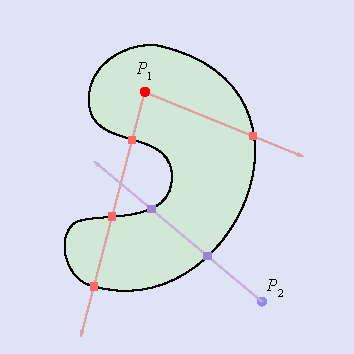
\includegraphics[width=0.5\textwidth]{inner_outer_pc.pdf}
    \bicaption[采样点的位置测试]{采样点的位置测试。自位于模型内部的采样点发出测试光线,与模型交点的个数一般为奇数,除非出现至少以此相切的情况;而自模型外部的采样点发出测试光线,与模型交点的个数一般为偶数}[Position test for sample points]{Position test for sample points. The number of intersection of the mesh boundary  and a ray emitted from an inner point should be odd, and the number of intersection of the mesh boundary and a ray emitted from a outer point should be even}
    \label{fig:pc_inout}
\end{figure}

编码器的输入是点云渲染到多个视角的深度图,因此在训练时可以将渲染过程进行预处理,以节省训练时间。对每个模型在单位球上采样270个相机位置,并渲染相应视角的点云深度图,为了保持深度图的浮点精度,采用EXR格式存储深度图文件。这样做还可以使得在训练来自一个点云不同视角的投影时,可以多次采样模型的测试点集和分类标签,使得单个模型有了更多的点集采样,有助于隐函数模块对真实几何的逼近。

\subsection{点云噪声的模拟}
与实际场景中扫描得到的真实点云相比,从三角面片上采样得到的点云不仅采样均匀,而且没有噪声和遮挡造成的空洞,在这样的数据上训练出的隐函数模块对真实数据的响应会差很多,因此需要模拟产生出噪声并叠加到采样点云上。主要考虑三种噪声模型,首先是对点云中各个点添加位置扰动,比对实际深度传感器的噪声数据,对归一化后的点云添加了方差为0.002的高斯扰动;第二种扰动为不均匀采样,先将同一个模型的面片随机分为30组,对每组面片按照面积比例,采样不同密度的点,再把所有采样点合起来作为最终的点云;第三种噪声考虑遮挡变化造成的空洞,在每个模型上随机选取20个点,采用宽度优先搜索(BFS,breadth first search)记录点周围若干步以内的面片,并将其删去,在余下的模型上再采样点云。图\ref{fig:pc_hole} 展示了步长为2时面片搜索的示例。
\begin{figure}[!htbp]
    \centering
    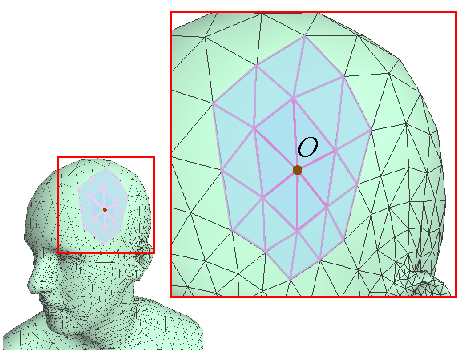
\includegraphics[width=0.6\textwidth]{hole_pc.pdf}
    \bicaption[面片上空洞的模拟]{面片上空洞的模拟。点$O$为采样的中心点,以两步为例,标识出了可达区域内的面片。}[Simulation of hole on the mesh]{Simulation of hole one the mesh. $O$ is one of the random samples. If the step number is two, the accessible triangles are marked.}
    \label{fig:pc_hole}
\end{figure}

\subsection{网络的训练与测试}
由于对点云的深度图进行了预渲染,训练的第一阶段仅包含单视角情况。一组训练数据就包含单视角的点云深度图、相机参数、对应模型的采样点集和各点的二分类标签。编码器对深度图进行编码,采样点投影到深度图得到插值的特征向量,并利用隐函数预测二分类的结果。在单视角训练结束之后,才进行多视角的数据进行调优,调优过程只需要2--3轮迭代就能收敛到较好的结果。这种渐进式增加视角数量的策略,提高了训练效率和泛化性能。

在测试的时候,对于输入点云,投影过程与训练过程无异。差异在于点采样的方式,由于测试时的目标是最终提取出面片,因此测试时按照规则三维网格进行采样。给定网格分辨率后对每个格点进行投影、采样特征向量以及预测隐函数值的过程,最终就可以通过marching cubes等方式提出面片。为了提高网格的预测效率,可以采用八叉树加速,对当前层级八个顶点分类结果一样的体素,就无须再继续细分下去,当然这样的剪枝有一定概率会在粗粒度时将整个几何丢失。

\section{本章小结}
本章介绍了以隐函数表达几何的同时基于多视角投影的点云重建算法部分。点云经投影和编码后得到特征,空间中的任意点从点云的特征上插值出自己的特征向量,代表隐函数的MLP继而将特征向量映射成隐函数值。训练过程中,特殊的点集采样策略提高了隐函数的逼近效果,并且通过模拟叠加噪声来提高鲁棒性,而两阶段渐进增加视角数量的策略缩减了训练时间。
\chapter{点云重建实验与分析}
本章介绍点云重建实验的细节、实验结果以及同其他方法的对比。实验在仿真数据和真实数据上均进行了验证。训练和定量的分析用到了两个人体数据集,一个是将动作捕捉序列拟合到SMPL参数化模型\citep{loper2015smpl}上生成的人体模型数据,另一个是真实人体通过多视角重建技术扫描得到的Twindom数据集。本方法与传统方法\citep{kazhdan2006, kazhdan2013}以及最新的基于深度学习的点云重建方法\citep{Chibane_2020_CVPR}进行了比较。实验证明新方法的鲁棒性在视觉效果和定量指标方面都优于这些方法。为了测试泛化性能,还进行了两个数据集之间的交叉测试实验。
真实数据由Kinect Azure搭建的采集系统获取,实验结果说明与传统方法相比,本方法具有良好的鲁棒性和泛化性能。

\section{实验环境和设置}
主机为64位x86架构机器,使用单张NVIDIA TITAN X显卡。网络使用PyTorch框架实现,可导渲染模块使用Pytorch3D实现。SMPL数据集的人体模型具有不同的姿态和形状,但是身体表面光滑,没有如衣服褶皱等高频信息,在所有的动作序列中采样导出了800个人体模型,所有模型具有同样的拓扑。Twindom数据集的人体模型姿态多为静态站立,由于采用多视角重建的方法恢复几何,衣服等几何细节保留逼真。从中随机挑出1200个模型,包括多种不同的复杂衣服、发型和形态。单个原始Twindom模型的顶点数量多达50万的量级,需要首先进行简化,将其顶点数量降到10万以下,同时严格保持模型质量几乎不受损。对于所有数据集,每个模型上采样点云的点数为20000,空间点集的采样数为5000。训练SMPL数据集和Twindom数据集的时间均在12小时左右,这包括了第一阶段的单视角训练和第二阶段的多视角调优。

\section{量化结果的比较}
在SMPL数据集和Twindom数据集,再加上各自模拟噪声产生的共四个数据集上,对比测试了单视角训练和多视角调优的效果,同时还对比了泊松重建和IFnet的表现。定量指标采用点云重建结果到真实模型的距离来衡量。给定点云$P$重建得到的几何$M_P$,对其上各顶点$v$,计算$v$到真实模型表面$M$的最近距离并求其均值,如公式(\ref{eq:pc_measure})所示。其中$|M_p|$表示重建出的几何包含的顶点数目。
\begin{equation} \label{eq:pc_measure}
    \adddotsbeforeeqnnum%
    D = \frac{1}{|M_p|}\sum_{v \in M_p} \|v - \mathrm{argmin}_{u\in M}\|v - u\|_2\|_2^2
\end{equation}

表\ref{tab:pc_measure}展示了依照此度量计算出的各个方法在数据集上的表现。可以看出,在没有噪声的情况下,泊松重建要明显优于深度学习的方法,这是因为点云的均匀采样如实反映出了模型的几何信息。然而在加入噪声后,泊松重建的结果会严重受到噪声影响,相反数据驱动的方法能够从训练数据中学习到去噪与补全缺损的方法,具有很好的鲁棒性。同时本方法采取的多视角投影提取几何信息的方式比直接从点云周围提取信息的IFnet表现更好。
\begin{table}[!htbp]
\bicaption[四个数据集上重建误差对比]{四个数据集上重建误差对比。Ours-s表示单视角训练结果,Ours-m表示多视角调优后的结果。真实模型尺度被缩放到单位1之内,距离值越小,重建效果越好。结果数据$\times 10^3$。}[Reconstruction loss of all methods on four datasets]{Reconstruction loss of all methods on four datasets. Ours-s is trained with single view supervision and Ours-m is refined with multi-view setting. The ground-truth models are scaled to uniform sphere. Smaller value implies better performance. Results $\times 10^3$.}
\label{tab:pc_measure}
\centering
\footnotesize% fontsize
\setlength{\tabcolsep}{4pt}% column separation
\renewcommand{\arraystretch}{0.9}%row space 
\begin{tabular}{c c c c c}
\hline\noalign{\smallskip}
Method  & Poisson & IFnet & Ours-s & Ours-m \\
\noalign{\smallskip}
\hline
\noalign{\smallskip}
SMPL   & \textbf{0.43} & 2.56 & 3.49 & 0.81 \\
SMPL+Noise & 1.34 & 1.73 & \textbf{1.17} & \textbf{0.92}\\
Twindom & \textbf{1.02} & 2.84 & 2.89 & 1.97 \\
Twindom+Noise & 3.43 & 2.74 &\textbf{1.84} & \textbf{1.36}\\
\hline
\end{tabular}
\end{table}

对比本方法在单视角训练和多视角调优的结果,可以发现经过多视角调优之后在各个数据集上的重建效果都会更好。SMPL数据集和Twindom数据集在单视角下,训练数据中加入噪声之后重建效果在数据上反而比不加噪声的时候表现更优,这可能是由于在添加噪声的情况下去噪和补洞操作都倾向于向均值回归,使得重建出的模型到真实模型的距离变小。

\section{可视化结果的比较}
图\ref{fig:pc_visual}展示了不同方法在两个数据集上的重建结果示例。SMPL
数据集的人体比较光滑,没有衣服纹理,而Twindom数据集的衣服纹理和头发细节更丰富。泊松重建对于细小结构例如手指等在采样密度不够的时候无法正确计算法向,因而无法准确重建相应结构。本方法的单视角重建结果能够恢复出大概的人体形状,即便无法恢复细节,也能大概补全出正确的轮廓,而经过多视角调优后能够获得更加精细的重建结果,对于比较精细的几何结构也取得了比传统方法更好的效果。

\begin{figure}
    \centering
    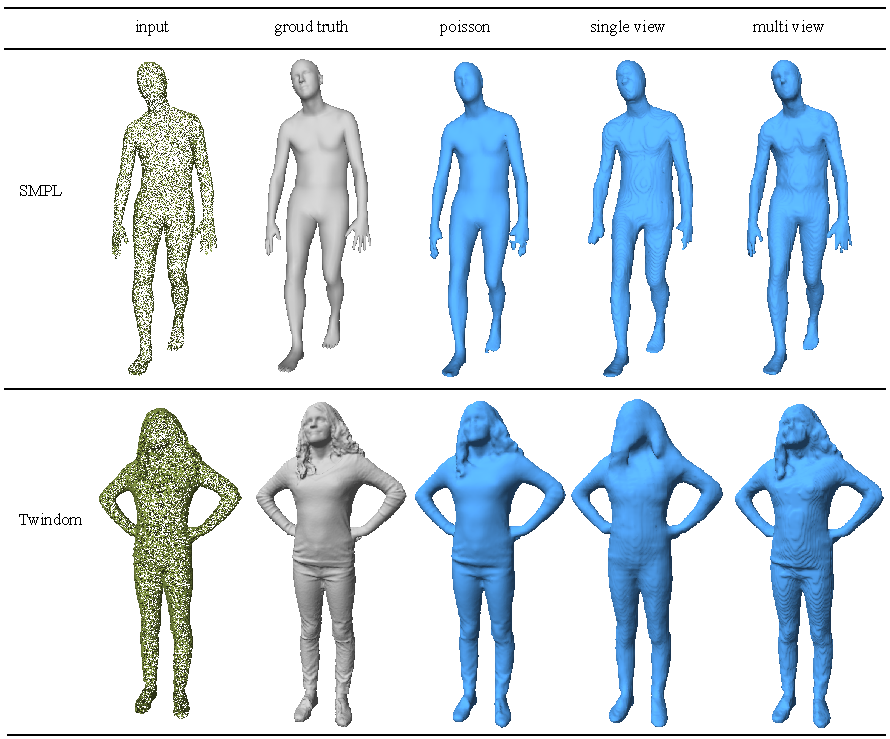
\includegraphics[width=\textwidth]{visual_result_pc.pdf}
    \bicaption[各方法在两个数据集上的点云重建结果对比]{各方法在两个数据集上的点云重建结果对比。单视角表示仅经过单视角训练,多视角 表示经过多视角调优后的结果。}[Results of different methods on SMPL and Twindom dataset]{Results of different methods on SMPL and Twindom dataset. “Single view” indicates the network is trained with single-view supervision only and "multi view" indicates the network is refined with multi-view setting.}
    \label{fig:pc_visual}
\end{figure}


\begin{figure}
    \centering
    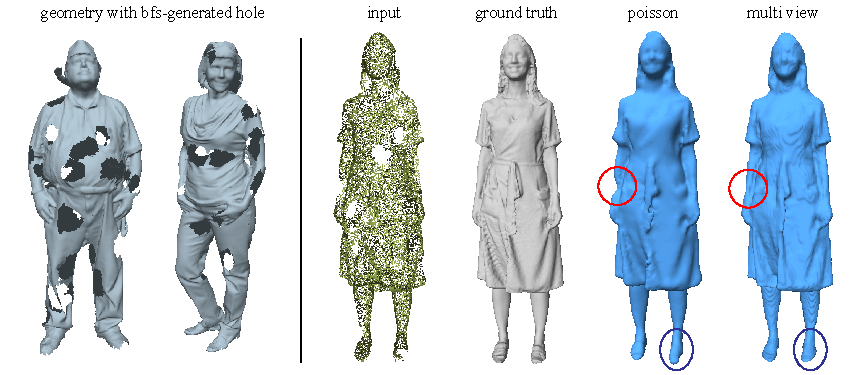
\includegraphics[width=\textwidth]{noise_pc.pdf}
    \bicaption[叠加模拟噪声后各方法的重建效果对比]{叠加模拟噪声后各方法的重建效果对比。圆圈区域显示了传统重建方法无法恢复而新方法能够正确推测并补全缺损的情况。}[Results of different methods when adding noise to geometry]{Results of different methods when adding noise to geometry. The circles indicates cases traditional methods failed to reconstruct while our method generalizes well.}
    \label{fig:pc_noise}
\end{figure}

\begin{figure}
    \centering
    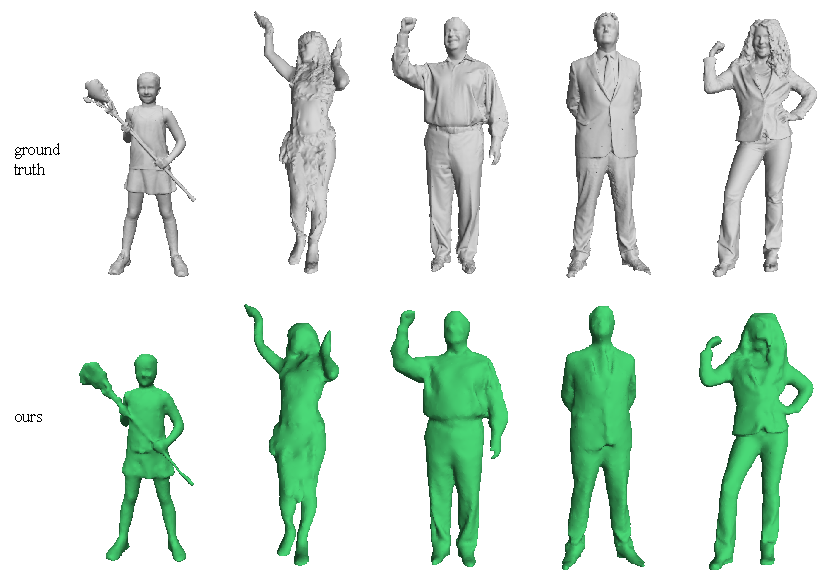
\includegraphics[width=\textwidth]{more_twindom_results.pdf}
    \bicaption[更多Twindom上的结果]{更多Twindom数据集上的结果。第一行为真实模型,第二行为本方法在Twindom数据集上的结果}[More results of Twindom dataset]{More results of Twindom dataset. The first line shows the ground truth data, the second line shows our results.}
    \label{fig:pc_more_twindom}
\end{figure}

图\ref{fig:pc_noise}展示了叠加模拟噪声的可视化结果。左边展示了Twindom训练集上通过BFS生成的空洞,右边对比了在测试数据上不同方法的结果。泊松重建由于缺乏数据先验,在较大面积缺损的情况下,从点云重建出的几何出现明显的瑕疵,而新方法在训练过程中对噪声和缺损有了先验,在测试数据上能保持较好的鲁棒性和泛化性,注意测试用的数据在训练过程中网络并未见过。

\section{数据集的交叉测试对比}
\begin{figure}[!htbp]
    \centering
    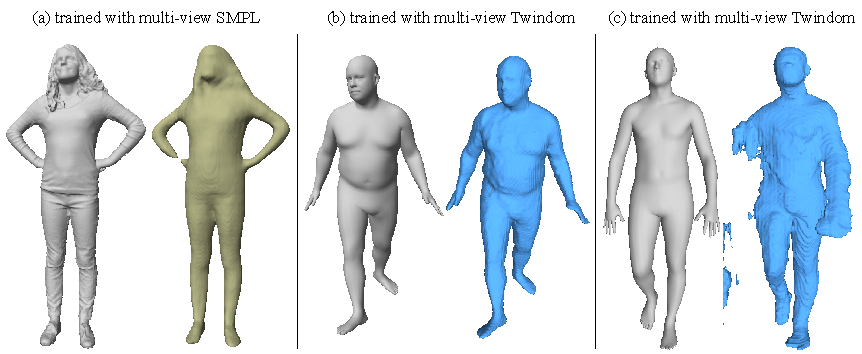
\includegraphics[width=\textwidth]{dataset_cross_pc.pdf}
    \bicaption[SMPL和Twindom交换测试集的结果对比]{SMPL和Twindom交换测试集的结果对比。(a)中模型在SMPL上多视角训练,在Twindom上多视角测试;(b)中模型在Twindom上多视角训练,在SMPL上多视角测试;(c)中模型在Twindom上多视角训练,在SMPL上单视角测试。}[Results of exchanging testing data on SMPL and Twindom dataset]{Results of exchanging testing data on SMPL and Twindom dataset. (a) The model is trained on SMPL (multi-view) and test on Twindom (multi-view); (b) The model is trained on Twindom (multi-view) and test on SMPL (multi-view); (c) The model is trained on Twindom (multi-view) and test on SMPL (single view).}
    \label{fig:pc_data_cross}
\end{figure}
为了比较隐函数在不同数据集上的表现差异以及验证网络的泛化性能,在SMPL和Twindom数据上进行了交叉测试,即用一个数据集的测试数据测试在另一个数据集上训练过的模型。图\ref{fig:pc_data_cross}展示了测试结果,当模型在SMPL数据集上训练之后,Twindom上的重建结果会过于平滑,衣服、头发和面部的几何细节明显丢失。当模型先在Twindom数据集上训练后,SMPL数据集的重建结果增加了部分细节,但是同时也引入了一些多余的细节,原本光滑的皮肤位置多出了很多褶皱。值得注意的是Twindom上经过多视角调优的网络,在SMPL上进行单视角测试时,出现了过多的噪声,甚至无法恢复出基本的形状信息,这说明隐函数对几何细节的学习和对噪声的容忍是存在权衡的,当数据倾向于表达更多细节时,隐函数模块更容易过拟合以保证丰富的细节。



\section{真实数据的测试结果}
采集系统由六个Kinect Azure设备构成,大致分布在一个直径为3米的圆周上,环绕着中间的拍摄物体,能够同步采集RGBD数据流。相机的位置参数通过预标定过程获得。采集得到的深度图充斥着噪声和由于遮挡变化导致的空洞,如图\ref{fig:pc_kinect_depth}所示。
\begin{figure}[!htbp]
    \centering
    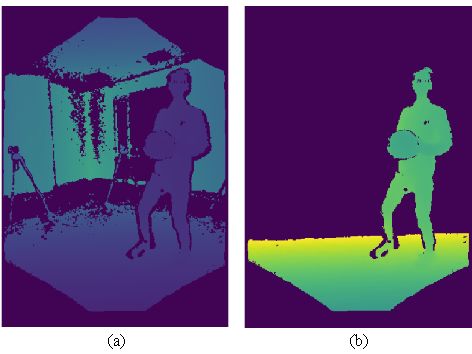
\includegraphics[width=0.6\textwidth]{kinect_depth.pdf}
    \bicaption[Kinect深度图的原始输入及预处理]{Kinect深度图的原始输入及预处理。(a)Kinect Azure原始深度图; (b)预处理结果。}[Raw Kiect depth map and results after pre-processing]{Raw Kiect depth map and results after pre-processing. (a) raw output of Kinect Azure; (b) result after pre-processing.}
    \label{fig:pc_kinect_depth}
\end{figure}
同时各个相机的标定过程产生的误差使得深度图无法完全对齐,图\ref{fig:pc_kinect_pointcloud}展示了从六个相机直接融合得到的点云,放大部分强调了三个导致点云质量差的主要原因:遮挡造成的空洞,标定误差造成的不对齐和离群噪声点。鉴于本方法对输入点云首先要投影到各个视角得到深度图,这使得Kinect采集到的深度图刚好可以直接作为编码器的输入。

图\ref{fig:pc_kinect_result}展示了重建结果。在获取的单帧点云质量较差的情况下,泊松重建无法处理噪声,所有的标定误差和噪声毛刺在重建结果中都依然存在,放大的局部细节中头部点云的大片空洞几何显得杂乱。而本方法使用了Twindom上预训练的模型,在噪声比较严重的情况下,保持了基本的形状和几何的平滑度,对于头部相机没有采到的区域,能够合理补全出头部形状,虽然模型本身有些过度平滑,但考虑到噪声和细节的权衡,得到的结果比传统方法明显更能让人接受。

\section{本章小结}

本章介绍了多视角投影结合隐函数的点云重建方法的实验结果。通过在SMPL数据集和Twindom 数据集上的测试,验证了方法的有效性。通过与其他方法的定量和观感上的对比,说明了本方法重建质量的优越性,尤其是对噪声和空洞等瑕疵的鲁棒性。通过在真实kinect数据上的测试,说明了新方法的泛化性和鲁棒性。

\begin{figure}[!htbp]
    \centering
    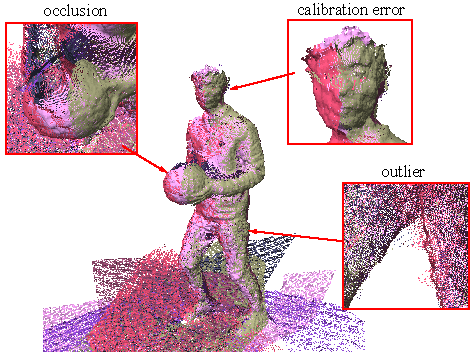
\includegraphics[width=0.7\textwidth]{kinect_pointcloud.pdf}
    \bicaption[六相机融合点云]{六相机融合点云。不同颜色代表来自不同相机的点云。放大部分展示了三个影响点云质量的因素。}[Raw pointclouds directly fused from six cameras]{Raw pointclouds directly fused from six cameras. Different color indicates the part of points are from different cameras. The three closeups shows the main cause of the artifacts.}
    \label{fig:pc_kinect_pointcloud}
\end{figure}

\begin{figure}[!htbp]
    \centering
    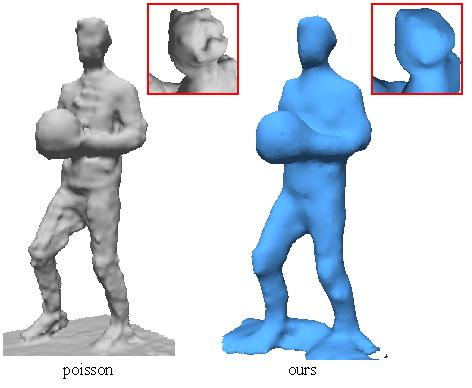
\includegraphics[width=0.65\textwidth]{kinect_result.pdf}
    \bicaption[Kinect数据的重建结果对比]{Kinect数据的重建结果对比。左边是泊松重建的结果,右边是本方法在Twindom上训练后对kinect数据的重建结果。}[Reconstruction results of Kinect data]{Reconstruction results of Kinect data. The left is result of poisson reconstruction, and the right is the results of our method trained with Twindom dataset.}
    \label{fig:pc_kinect_result}
\end{figure}
\chapter{总结与展望}
本文研究了隐式几何表达与深度学习框架的结合形式,首先通过编码器结构将输入转化到特征空间,再以特定的隐式几何表达作为中间件,根据不同需求计算输出。本文通过自由视角插值和点云重建这两个具体任务,讨论了该框架融合先验知识和数据驱动的优势及潜力。

环形三相机插值方法能够对大致分布在圆环上的三个相机的图片进行连续插值,革新了原先的两相机之间的视角插值模型。通过环形校正将三张图片对齐到标准圆弧上,并将图片插值过程全部以可导的神经网络表达。选择视差作为几何表达,并辅以可见区域信息。网络的编码器模块提取彩色图片中的特征后,解码器预测视差和可见区域信息,最终渲染模块根据视差的几何意义生成新视角的图片。在一般物体模型和人体模型数据上的实验表明,本方法的新视角生成效果优于其他方法,能够较好地消除遮挡造成的歧义。利用新的视角插值方法能够轻易地生成“子弹时间”特效。

多视角投影的点云重建方法能从粗糙的点云数据中恢复几何,针对点云数据的噪声以及空洞缺陷,能够较好地去噪和补全。点云经过多视角投影得到深度图,深度图经过编码器得到特征张量。在这个任务中以隐函数作为几何的表达形式,能对空间任意点预测隐函数值,最后提取隐函数的等值面。误差函数将几何误差的衡量表达为对采样点的分类误差,将隐函数的拟合与点采样结合起来。在两个人体数据集上的实验表明,新方法处理噪声和空洞的能力明显优于传统方法,多视角投影的编码方式不仅能提取特征,还能利用不同尺度的信息对点云在2D上进行去噪和补全。在真实的Kinect数据上的实验证明了新方法良好的泛化性能。

通过视角插值和点云重建这两个任务,验证了将隐式几何形式内嵌到深度学习框架这一想法的可行性,通过对数据集的选择,也能实现将数据先验和知识先验结合的目标,但是从实验中也发现了一些明显的不足,这主要集中在生成的数据质量、可编辑性以及可解释性方面。

在视角插值任务中,在单张11G显卡的限制下,生成图片尺寸最高只能达到512分辨率,这不满足当前手机等显示设备的高清要求,同时生成图片仍然存在细节模糊不清的缺点。在连续生成图片序列时,有时会出现某一帧质量明显下降,甚至出现明显瑕疵的情况。与传统确定性算法不同,网络生成的数据出现瑕疵时,很难精确定位到具体网络参数,是神经网络可编辑性差的一个体现。

在点云重建任务中,生成的模型往往趋于平滑,对于精细的细节如手指、头发丝以及面部五官细节等,无法获得精确几何。提取隐函数的等值面时,规范网格的分辨率一般为256,最高可达512,但是提取单个模型的时间将需要几分钟,同时提取算法无法根据真实几何是否具备高频细节,自适应地调节需要的采样粒度。对于人体模型,当头发较长,并且距离面部较近时,点云重建结果中头发与面部往往会糊成一团,失去大量细节,对不同的模型表现会有所差异。对这样的问题,同样很难精确定位到网络参数并对其进行编辑。

这些在不同应用中表现出的问题之间存在着明显的相关性。生成的数据质量上呈现出的模糊和细节缺失的问题,应与编码器以卷积操作为主有关。而无规律出现瑕疵的情形,在几乎所有的深度学习任务中都存在。针对细节缺失的问题,需要考虑改良卷积操作,目前有一些工作用基于光线采样的表达形式替换了全图卷积操作,有望能提升细节。针对可编辑性的操作,同样需要改进特征的表达方式,很多产生式模型的工作都涉及讨论隐编码(latent code)对特征空间的结构和可编辑性的作用,借鉴这方面的工作有望能厘清特征空间的更多性质,从而在小的变化范围内定位瑕疵的原因并试图改进。


%---------------------------------------------------------------------------%
% main content
%-
%-> Appendix
%-
\cleardoublepage%
\appendix% initialize the environment
% \chapter{中国科学院大学学位论文撰写要求}

学位论文是研究生科研工作成果的集中体现,是评判学位申请者学术水平、授予其学位的主要依据,是科研领域重要的文献资料。根据《科学技术报告、学位论文和学术论文的编写格式》(GB/T 7713-1987)、《学位论文编写规则》(GB/T 7713.1-2006)和《文后参考文献著录规则》(GB7714—87)等国家有关标准,结合中国科学院大学(以下简称“国科大”)的实际情况,特制订本规定。

\section{论文无附录者无需附录部分}

\section{测试公式编号 \texorpdfstring{$\Lambda,\lambda,\theta,\bar{\Lambda},\sqrt{S_{NN}}$}{$\textLambda,\textlambda,\texttheta,\bar{\textLambda},\sqrt{S_{NN}}$}} \label{sec:testmath}

\begin{equation} \label{eq:appedns}
    \adddotsbeforeeqnnum%
    \begin{cases}
        \frac{\partial \rho}{\partial t} + \nabla\cdot(\rho\Vector{V}) = 0\\
        \frac{\partial (\rho\Vector{V})}{\partial t} + \nabla\cdot(\rho\Vector{V}\Vector{V}) = \nabla\cdot\Tensor{\sigma}\\
        \frac{\partial (\rho E)}{\partial t} + \nabla\cdot(\rho E\Vector{V}) = \nabla\cdot(k\nabla T) + \nabla\cdot(\Tensor{\sigma}\cdot\Vector{V})
    \end{cases}
\end{equation}
\begin{equation}
    \adddotsbeforeeqnnum%
    \frac{\partial }{\partial t}\int\limits_{\Omega} u \, \mathrm{d}\Omega + \int\limits_{S} \unitVector{n}\cdot(u\Vector{V}) \, \mathrm{d}S = \dot{\phi}
\end{equation}
\[
    \begin{split}
        \mathcal{L} \{f\}(s) &= \int _{0^{-}}^{\infty} f(t) e^{-st} \, \mathrm{d}t, \ 
        \mathscr{L} \{f\}(s) = \int _{0^{-}}^{\infty} f(t) e^{-st} \, \mathrm{d}t\\
        \mathcal{F} {\bigl (} f(x+x_{0}) {\bigr )} &= \mathcal{F} {\bigl (} f(x) {\bigr )} e^{2\pi i\xi x_{0}}, \ 
        \mathscr{F} {\bigl (} f(x+x_{0}) {\bigr )} = \mathscr{F} {\bigl (} f(x) {\bigr )} e^{2\pi i\xi x_{0}}
    \end{split}
\]

mathtext: $A,F,L,2,3,5,\sigma$, mathnormal: $A,F,L,2,3,5,\sigma$, mathrm: $\mathrm{A,F,L,2,3,5,\sigma}$.

mathbf: $\mathbf{A,F,L,2,3,5,\sigma}$, mathit: $\mathit{A,F,L,2,3,5,\sigma}$, mathsf: $\mathsf{A,F,L,2,3,5,\sigma}$.

mathtt: $\mathtt{A,F,L,2,3,5,\sigma}$, mathfrak: $\mathfrak{A,F,L,2,3,5,\sigma}$, mathbb: $\mathbb{A,F,L,2,3,5,\sigma}$.

mathcal: $\mathcal{A,F,L,2,3,5,\sigma}$, mathscr: $\mathscr{A,F,L,2,3,5,\sigma}$, boldsymbol: $\boldsymbol{A,F,L,2,3,5,\sigma}$.

vector: $\Vector{\sigma, T, a, F, n}$, unitvector: $\unitVector{\sigma, T, a, F, n}$

matrix: $\Matrix{\sigma, T, a, F, n}$, unitmatrix: $\unitMatrix{\sigma, T, a, F, n}$

tensor: $\Tensor{\sigma, T, a, F, n}$, unittensor: $\unitTensor{\sigma, T, a, F, n}$ 

\section{测试生僻字}

霜蟾盥薇曜灵霜颸妙鬘虚霩淩澌菀枯菡萏泬寥窅冥毰毸濩落霅霅便嬛岧峣瀺灂姽婳愔嫕飒纚棽俪緸冤莩甲摛藻卮言倥侗椒觞期颐夜阑彬蔚倥偬澄廓簪缨陟遐迤逦缥缃鹣鲽憯懔闺闼璀错媕婀噌吰澒洞阛闠覼缕玓瓑逡巡諓諓琭琭瀌瀌踽踽叆叇氤氲瓠犀流眄蹀躞赟嬛茕頔璎珞螓首蘅皋惏悷缱绻昶皴皱颟顸愀然菡萏卑陬纯懿犇麤掱暒 墌墍墎墏墐墒墒墓墔墕墖墘墖墚墛坠墝增墠墡墢墣墤墥墦墧墨墩墪樽墬墭堕墯墰墱墲坟墴墵垯墷墸墹墺墙墼墽垦墿壀壁壂壃壄壅壆坛壈壉壊垱壌壍埙壏壐壑壒压壔壕壖壗垒圹垆壛壜壝垄壠壡坜壣壤壥壦壧壨坝塆圭嫶嫷嫸嫹嫺娴嫼嫽嫾婳妫嬁嬂嬃嬄嬅嬆嬇娆嬉嬊娇嬍嬎嬏嬐嬑嬒嬓嬔嬕嬖嬗嬘嫱嬚嬛嬜嬞嬟嬠嫒嬢嬣嬥嬦嬧嬨嬩嫔嬫嬬奶嬬嬮嬯婴嬱嬲嬳嬴嬵嬶嬷婶嬹嬺嬻嬼嬽嬾嬿孀孁孂娘孄孅孆孇孆孈孉孊娈孋孊孍孎孏嫫婿媚嵭嵮嵯嵰嵱嵲嵳嵴嵵嵶嵷嵸嵹嵺嵻嵼嵽嵾嵿嶀嵝嶂嶃崭嶅嶆岖嶈嶉嶊嶋嶌嶍嶎嶏嶐嶑嶒嶓嵚嶕嶖嶘嶙嶚嶛嶜嶝嶞嶟峤嶡峣嶣嶤嶥嶦峄峃嶩嶪嶫嶬嶭崄嶯嶰嶱嶲嶳岙嶵嶶嶷嵘嶹岭嶻屿岳帋巀巁巂巃巄巅巆巇巈巉巊岿巌巍巎巏巐巑峦巓巅巕岩巗巘巙巚帠帡帢帣帤帨帩帪帬帯帰帱帲帴帵帷帹帺帻帼帽帾帿幁幂帏幄幅幆幇幈幉幊幋幌幍幎幏幐幑幒幓幖幙幚幛幜幝幞帜幠幡幢幤幥幦幧幨幩幪幭幮幯幰幱庍庎庑庖庘庛庝庠庡庢庣庤庥庨庩庪庬庮庯庰庱庲庳庴庵庹庺庻庼庽庿廀厕廃厩廅廆廇廋廌廍庼廏廐廑廒廔廕廖廗廘廙廛廜廞庑廤廥廦廧廨廭廮廯廰痈廲廵廸廹廻廼廽廿弁弅弆弇弉弖弙弚弜弝弞弡弢弣弤弨弩弪弫弬弭弮弰弲弪弴弶弸弻弼弽弿彖彗彘彚彛彜彝彞彟彴彵彶彷彸役彺彻彽彾佛徂徃徆徇徉后徍徎徏径徒従徔徕徖徙徚徛徜徝从徟徕御徢徣徤徥徦徧徨复循徫旁徭微徯徰徱徲徳徴徵徶德徸彻徺忁忂惔愔忇忈忉忔忕忖忚忛応忝忞忟忪挣挦挧挨挩挪挫挬挭挮挰掇授掉掊掋掍掎掐掑排掓掔掕挜掚挂掜掝掞掟掠采探掣掤掦措掫掬掭掮掯掰掱掲掳掴掵掶掸掹掺掻掼掽掾掿拣揁揂揃揅揄揆揇揈揉揊揋揌揍揎揑揓揔揕揖揗揘揙揤揥揦揧揨揫捂揰揱揲揳援揵揶揷揸揻揼揾揿搀搁搂搃搄搅搇搈搉搊搋搌搎搏搐搑搒摓摔摕摖摗摙摚摛掼摝摞摠摡斫斩斮斱斲斳斴斵斶斸旪旫旮旯晒晓晔晕晖晗晘晙晛晜晞晟晠晡晰晣晤晥晦晧晪晫晬晭晰晱晲晳晴晵晷晸晹晻晼晽晾晿暀暁暂暃暄暅暆暇晕晖暊暋暌暍暎暏暐暑暒暓暔暕暖暗旸暙暚暛暜暝暞暟暠暡暣暤暥暦暧暨暩暪暬暭暮暯暰昵暲暳暴暵
% appendix content
%-
%-> Backmatter: bibliography, glossary, index
%-
\backmatter% initialize the environment
\intotoc*{\cleardoublepage}{\bibname}% add link to toc
\bibliography{Biblio/ref}% bibliography
%---------------------------------------------------------------------------%
%->> Backmatter
%---------------------------------------------------------------------------%
\chapter{作者简历及攻读学位期间发表的学术论文与研究成果}

\section*{作者简历}

\noindent 2011年9月 --- 2015年6月,于清华大学自动化系获得学士学位。

\noindent 2015年9月 --- 2021年6月,于中国科学院上海微系统与信息技术研究所攻读硕士学位。

\section*{已发表(或正式接受)的学术论文:}

{
\setlist[enumerate]{}% restore default behavior
\begin{enumerate}[nosep]
    \item YANG YANG, JIN SHI, LIU RUIYANG, KANG SINGBING, YU JINGYI. Automatic 3D Indoor Scene Modeling From Single Panorama[C]//Proceedings of the IEEE Conference on Computer Vision and Pattern Recognition (CVPR), 2018.
    \item  JIN SHI, LIU RUIYANG, JI YU, YE JINWEI, YU JINGYI. Learning to Dodge A Bullet: Concyclic View Morphing via Deep Learning[C]//Proceedings of European Conference on Computer Vision (ECCV), 2018.
    \item 金石.多视角投影学习隐函数的点云重建方法[J/OL].重庆大学学报, 2021, xx(x):x-x.(审稿中)
\end{enumerate}
}

\section*{申请或已获得的专利:}

(无专利时此项不必列出)

\section*{参加的研究项目及获奖情况:}



\chapter[致谢]{致\quad 谢}\chaptermark{致\quad 谢}% syntax: \chapter[目录]{标题}\chaptermark{页眉}
\thispagestyle{noheaderstyle}% 如果需要移除当前页的页眉
%\pagestyle{noheaderstyle}% 如果需要移除整章的页眉

感谢我的研究生导师,论文指导老师,上海科技大学信息科学与技术学院虞晶怡教授,对我论文以及研究生生涯中的学术指导。感谢上海科技大学智能视觉中心的同学和老师们,在研究生期间对我学术和生活上的关心。还要感谢中科院上海微系统所的老师们,在我得以在上海科技大学得到学习的机会,以及在毕业论文方面给我的支持。

感谢与我一同合作科研项目的同学们,大家一起学习共同进步的拼搏时光,我将永远记住。在代码实现和撰写文章时,予我指点的各位师兄师姐,带领我一窥计算机视觉这个庞大领域的科研之道。

还要感谢上海科技大学教授我课程的各位老师们,这些在课堂上学习到的理论知识最终用在了科研工作和学习的方方面面。

最后感谢评阅论文的各位老师,为我的论文付出了宝贵的时间和精力,给我指导和建议。

再次向所有给我帮助、关爱我的亲人、师长、朋友,表示感谢。

\cleardoublepage[plain]% 让文档总是结束于偶数页,可根据需要设定页眉页脚样式,如 [noheaderstyle]
%---------------------------------------------------------------------------%
% other information
\end{document}
%---------------------------------------------------------------------------%

